\documentclass{beamer}\usepackage[]{graphicx}\usepackage[]{color}
% maxwidth is the original width if it is less than linewidth
% otherwise use linewidth (to make sure the graphics do not exceed the margin)
\makeatletter
\def\maxwidth{ %
  \ifdim\Gin@nat@width>\linewidth
    \linewidth
  \else
    \Gin@nat@width
  \fi
}
\makeatother

\definecolor{fgcolor}{rgb}{0.345, 0.345, 0.345}
\newcommand{\hlnum}[1]{\textcolor[rgb]{0.686,0.059,0.569}{#1}}%
\newcommand{\hlstr}[1]{\textcolor[rgb]{0.192,0.494,0.8}{#1}}%
\newcommand{\hlcom}[1]{\textcolor[rgb]{0.678,0.584,0.686}{\textit{#1}}}%
\newcommand{\hlopt}[1]{\textcolor[rgb]{0,0,0}{#1}}%
\newcommand{\hlstd}[1]{\textcolor[rgb]{0.345,0.345,0.345}{#1}}%
\newcommand{\hlkwa}[1]{\textcolor[rgb]{0.161,0.373,0.58}{\textbf{#1}}}%
\newcommand{\hlkwb}[1]{\textcolor[rgb]{0.69,0.353,0.396}{#1}}%
\newcommand{\hlkwc}[1]{\textcolor[rgb]{0.333,0.667,0.333}{#1}}%
\newcommand{\hlkwd}[1]{\textcolor[rgb]{0.737,0.353,0.396}{\textbf{#1}}}%
\let\hlipl\hlkwb

\usepackage{framed}
\makeatletter
\newenvironment{kframe}{%
 \def\at@end@of@kframe{}%
 \ifinner\ifhmode%
  \def\at@end@of@kframe{\end{minipage}}%
  \begin{minipage}{\columnwidth}%
 \fi\fi%
 \def\FrameCommand##1{\hskip\@totalleftmargin \hskip-\fboxsep
 \colorbox{shadecolor}{##1}\hskip-\fboxsep
     % There is no \\@totalrightmargin, so:
     \hskip-\linewidth \hskip-\@totalleftmargin \hskip\columnwidth}%
 \MakeFramed {\advance\hsize-\width
   \@totalleftmargin\z@ \linewidth\hsize
   \@setminipage}}%
 {\par\unskip\endMakeFramed%
 \at@end@of@kframe}
\makeatother

\definecolor{shadecolor}{rgb}{.97, .97, .97}
\definecolor{messagecolor}{rgb}{0, 0, 0}
\definecolor{warningcolor}{rgb}{1, 0, 1}
\definecolor{errorcolor}{rgb}{1, 0, 0}
\newenvironment{knitrout}{}{} % an empty environment to be redefined in TeX

\usepackage{alltt}

\def\currentCourse{Masterclass in Machine Learning}
\def\currentInstitute{Villiers-le-lac}
\def\currentLogo{../common_figs/logo_apt}
\def\currentDate{January 2022}
\def\currentChapter{Graph clustering and the Stochastic Bloc Model}


% THEME BEAMER
\usepackage{../beamer_theme}

\graphicspath{{figures/},{../common_figs/}}

\usepackage{multirow}
\usepackage{tikz}
\usepackage[vlined]{algorithm2e}

\pgfdeclareimage[width=.5cm]{computer}{computer.png}

% \usetikzlibrary{calc,shapes,backgrounds,arrows,automata,shadows,positioning}
% \tikzstyle{every state}=[fill=red,draw=none,scale=0.7,font=\small,text=white]
% \tikzstyle{every edge}=[-,shorten >=1pt,auto,thin,draw]
% \tikzstyle{alertstate}=[fill=bleu]
% \definecolor{genecolor}{RGB}{94,135,173}

\title{\currentCourse}

\subtitle{\huge\currentChapter\normalsize}

\institute{\currentInstitute}

\date{\currentDate}



\AtBeginSection{
  \begin{frame}<beamer>
    \frametitle{Outline}
    \framesubtitle{\insertpart}
    \tableofcontents[currentsection,currentsubsection, subsectionstyle=show/shaded/hide]  
  \end{frame}
}

\AtBeginSubsection{
  \begin{frame}<beamer>
    \frametitle{Outline}
    \framesubtitle{\insertpart}
    \tableofcontents[currentsection,currentsubsection, subsectionstyle=show/shaded/hide]  
  \end{frame}
}

\AtBeginSubsubsection{
  \begin{frame}<beamer>
    \frametitle{Outline}
    \framesubtitle{\insertpart}
    \tableofcontents[currentsection,currentsubsection, subsectionstyle=show/shaded/hide]  
  \end{frame}
}

\newcommand{\dotitlepage}{%
  \begin{frame}
    \titlepage
    \vfill
    \begin{center}
        \scriptsize\url{https://jchiquet.github.io/}
    \end{center}
    \vfill
    \includegraphics[width=2cm]{\currentLogo}\hfill
    \includegraphics[width=2.5cm]{logo_inrae}
  \end{frame}
  %
}

\newcommand{\dotoc}{%
  \begin{frame}
    \frametitle{Outline}
    \tableofcontents[currentsection,
    sectionstyle=show/show,
    subsectionstyle=hide]
  \end{frame}
  %
}

\usetikzlibrary{calc,shapes,backgrounds,arrows,automata,shadows,positioning}
\definecolor{mygreen}{RGB}{20, 176, 61}
\IfFileExists{upquote.sty}{\usepackage{upquote}}{}
\begin{document}

\dotitlepage

\begin{frame}[fragile]
  \frametitle{Setup and Reproducibility}
  
\begin{knitrout}\scriptsize
\definecolor{shadecolor}{rgb}{0.969, 0.969, 0.969}\color{fgcolor}\begin{kframe}
\begin{alltt}
\hlkwd{library}\hlstd{(tidyverse)} \hlcom{# data manipulation}
\hlkwd{library}\hlstd{(igraph)}    \hlcom{# graph manipulation}
\hlkwd{library}\hlstd{(sbm)}       \hlcom{# stochastic bloc model}
\hlkwd{library}\hlstd{(missSBM)}   \hlcom{# stochastic bloc model with missing data}
\hlkwd{library}\hlstd{(aricode)}   \hlcom{# clustering measures comparison}
\end{alltt}
\end{kframe}
\end{knitrout}



\end{frame}

\begin{frame}
  \frametitle{Outline}
  \tableofcontents
\end{frame}

%% ==========================================================================
\section{Motivations}
%% ==========================================================================

\begin{frame}
  \frametitle{Network data}

  \begin{block}{Recommandation system: Epinion}
Who-trust-whom online social network of a general consumer review site Epinions.com. Members of the site can decide whether to ''trust'' each other. 

\end{block}

\begin{block}{Social networks in ethnobiology}

A seed exchange network in Kenya is collected on a limited space area, where all the 155 farmers are interviewed. Farmers provide information about other farmers with whom they have interacted.

\end{block}

\begin{block}{Ecological networks: plant-pollinator network}
Interaction network between predefined sets of plants and pollinators, by direct observation.
\end{block}

\end{frame}

\begin{frame}[fragile]
  \frametitle{Companion data set: French political Blogosphere}

Single day snapshot of almost 200 political blogs automatically extracted the 14 October 2006 and manually classified by the "Observatoire Présidentielle" project.

\begin{knitrout}\scriptsize
\definecolor{shadecolor}{rgb}{0.969, 0.969, 0.969}\color{fgcolor}\begin{kframe}
\begin{alltt}
\hlkwd{data}\hlstd{(}\hlstr{"frenchblog2007"}\hlstd{,} \hlkwc{package} \hlstd{=} \hlstr{"missSBM"}\hlstd{)}
\hlstd{blog} \hlkwb{<-} \hlstd{frenchblog2007} \hlopt  \hlkwd{delete_vertices}\hlstd{(}\hlkwd{which}\hlstd{(}\hlkwd{degree}\hlstd{(frenchblog2007)} \hlopt{<=} \hlnum{1}\hlstd{))}
\hlkwd{summary}\hlstd{(blog)}
\end{alltt}
\begin{verbatim}
## IGRAPH 6fb607c UN-- 192 1431 -- 
## + attr: name (v/c), party (v/c)
\end{verbatim}
\begin{alltt}
\hlstd{party} \hlkwb{<-} \hlkwd{V}\hlstd{(blog)}\hlopt{$}\hlstd{party} \hlopt \hlkwd{as_factor}\hlstd{()}
\hlstd{party} \hlopt \hlkwd{table}\hlstd{()} \hlopt \hlstd{knitr}\hlopt{::}\hlkwd{kable}\hlstd{(}\hlstr{"latex"}\hlstd{)}
\end{alltt}
\end{kframe}
\begin{tabular}{l|r}
\hline
. & Freq\\
\hline
green & 9\\
\hline
right & 40\\
\hline
center-rigth & 32\\
\hline
left & 57\\
\hline
center-left & 11\\
\hline
far-left & 7\\
\hline
liberal & 25\\
\hline
analyst & 11\\
\hline
\end{tabular}

\end{knitrout}

\end{frame}

\begin{frame}[fragile]
  \frametitle{Visualization: graph view}

A visual representation of the network data with nodes colored according to the political party each blog belongs to is achieved as follows:

\begin{knitrout}\scriptsize
\definecolor{shadecolor}{rgb}{0.969, 0.969, 0.969}\color{fgcolor}\begin{kframe}
\begin{alltt}
\hlkwd{plot.igraph}\hlstd{(blog,}
  \hlkwc{vertex.color} \hlstd{= party,}
  \hlkwc{vertex.label} \hlstd{=} \hlnum{NA}
 \hlstd{)}
\end{alltt}
\end{kframe}
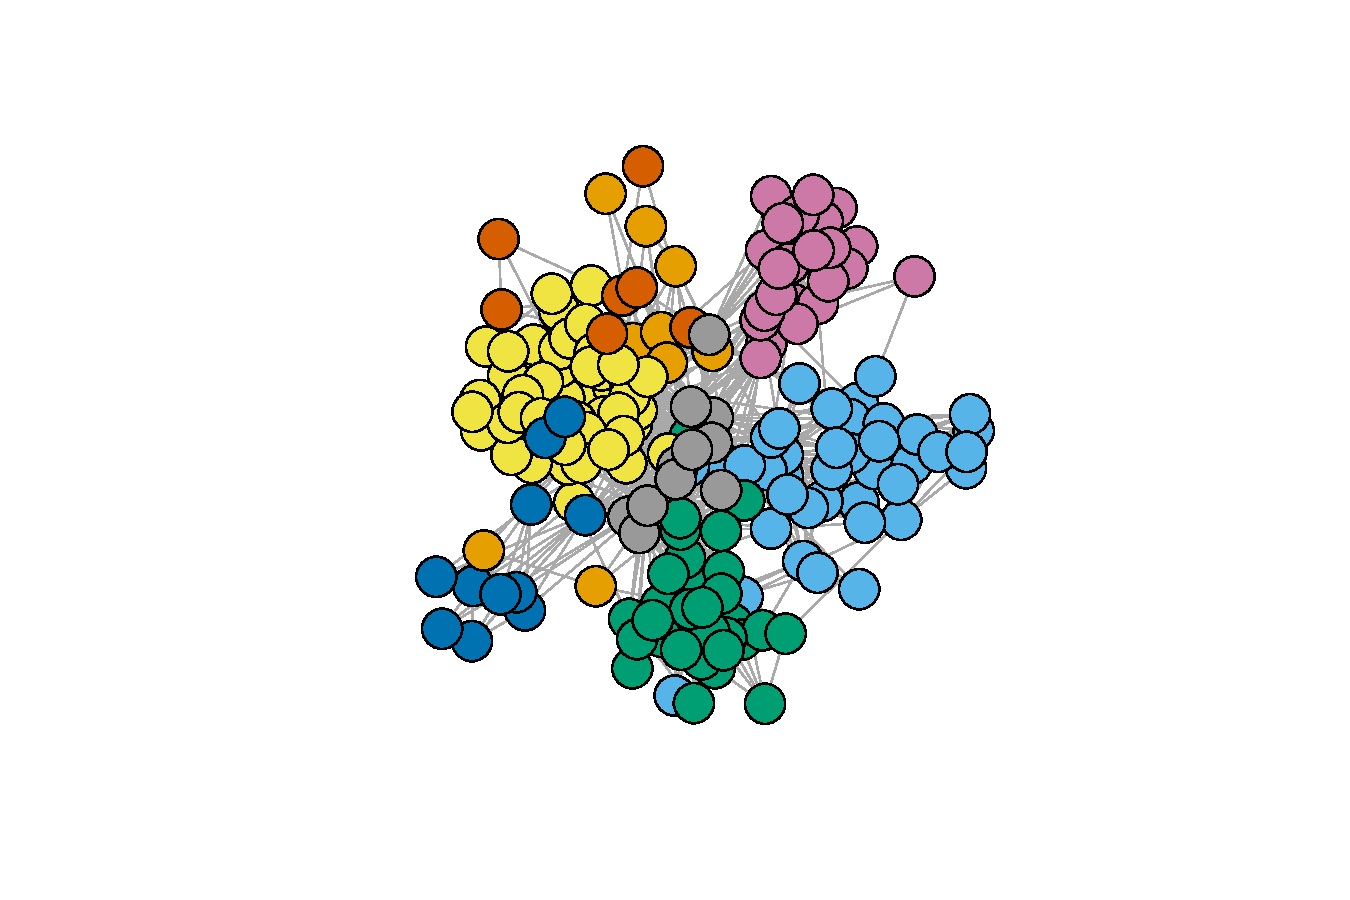
\includegraphics[width=.8\textwidth]{figures/frenchblog-igraph-plot-1} 
\end{knitrout}

\end{frame}

\begin{frame}[fragile]
  \frametitle{Visualization: graph view (advanced)}



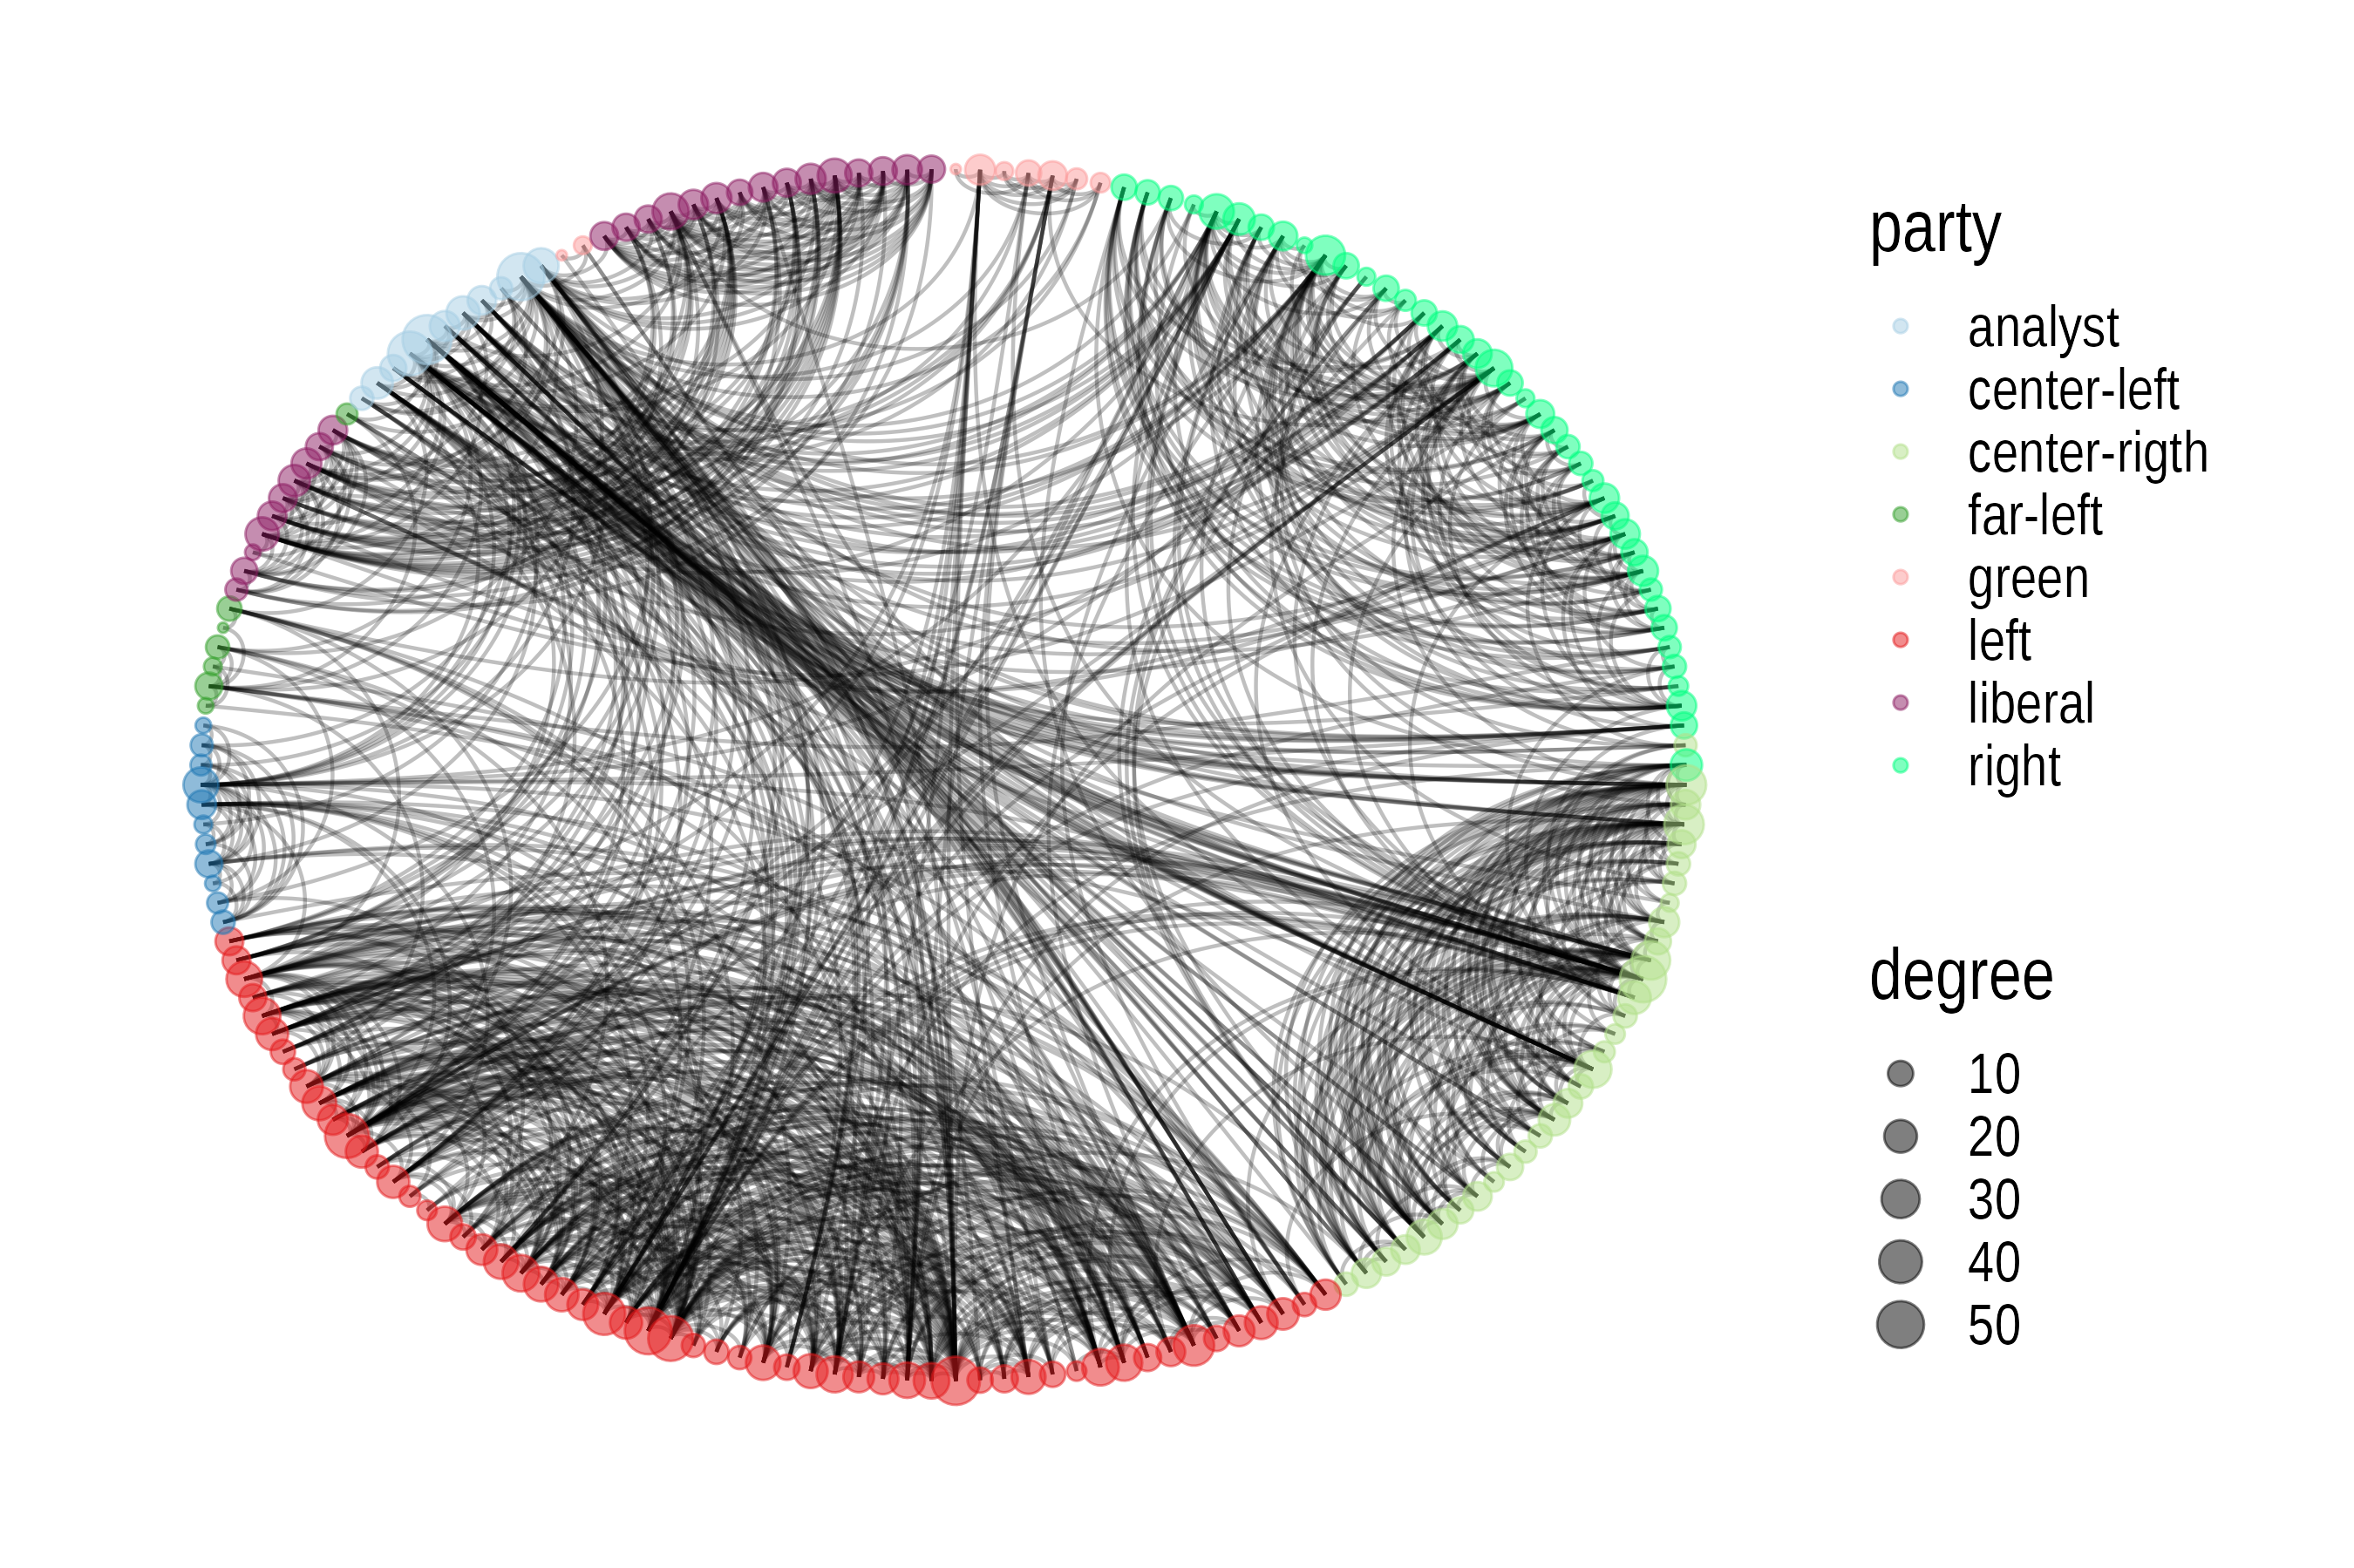
\includegraphics[height=.9\textheight]{figures/fancy_frenchblog2007.png}

\end{frame}

\begin{frame}[fragile]
  \frametitle{Visualization: matrix view}

\begin{knitrout}\scriptsize
\definecolor{shadecolor}{rgb}{0.969, 0.969, 0.969}\color{fgcolor}\begin{kframe}
\begin{alltt}
\hlstd{Y}  \hlkwb{<-} \hlkwd{as_adj}\hlstd{(blog,} \hlkwc{sparse} \hlstd{=} \hlnum{FALSE}\hlstd{)}
\hlstd{sbm}\hlopt{::}\hlkwd{plotMyMatrix}\hlstd{(}
  \hlstd{Y,} \hlkwc{dimLabels} \hlstd{=} \hlkwd{list}\hlstd{(}\hlstr{'blog'}\hlstd{,} \hlstr{"blog ordered per party"}\hlstd{),}
  \hlkwc{clustering} \hlstd{=} \hlkwd{list}\hlstd{(}\hlkwc{row} \hlstd{= party))}
\end{alltt}
\end{kframe}
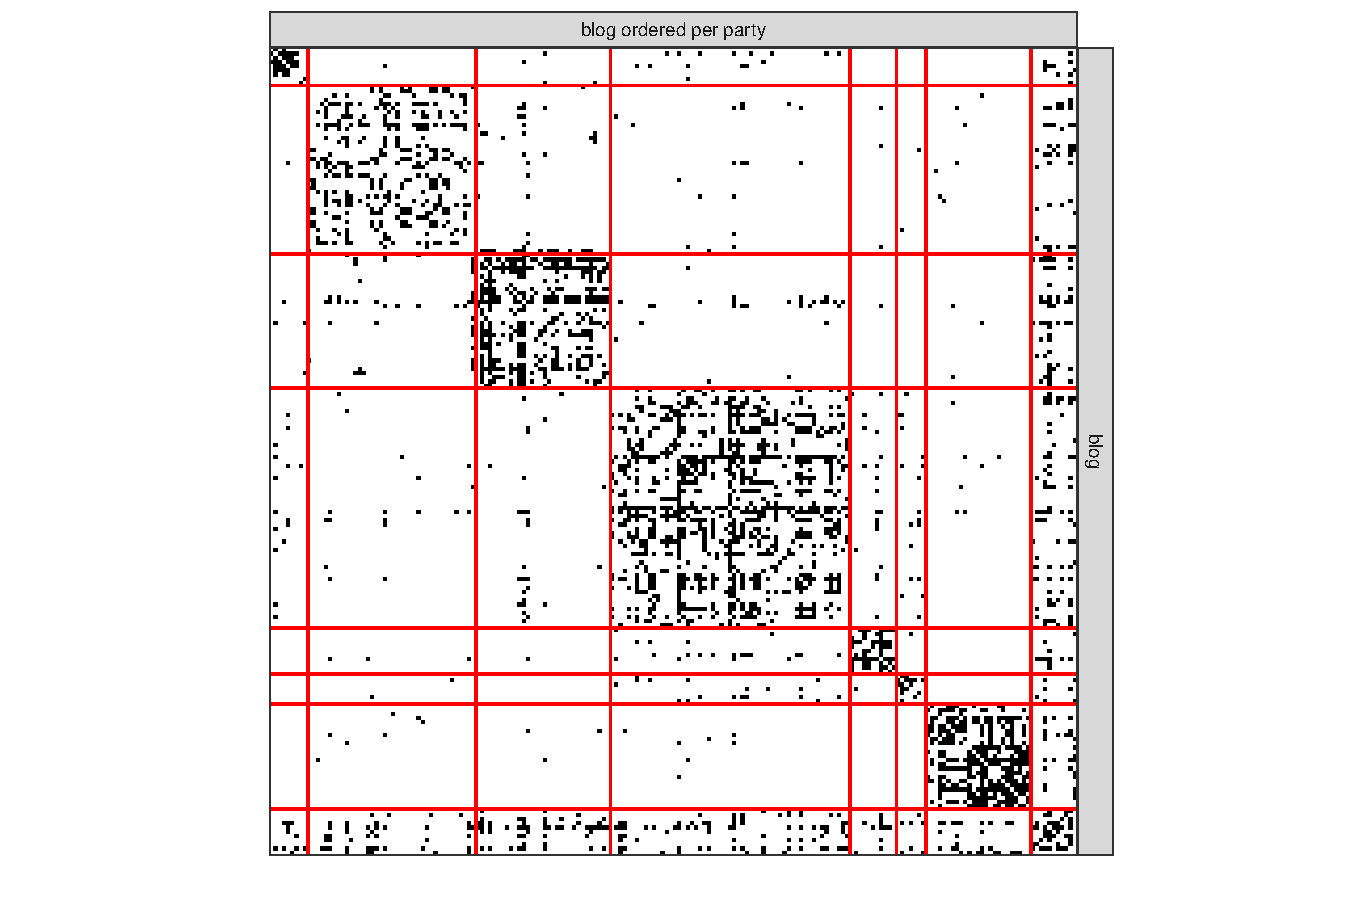
\includegraphics[width=.8\textwidth]{figures/unnamed-chunk-1-1} 
\end{knitrout}

\end{frame}

\begin{frame}
  \frametitle{Questions}

\begin{block}{Remarks}  
  
  \begin{itemize}
  
  \item  The pattern of connections between the nodes is highly related to the blog classification (political party). 
  
  \item The data may support a natural grouping of the node which is not necessarily related to a predefined classification
  
  \item Same remark holds for any kind of clustering and unsupervised leaning problem

  \end{itemize}
\end{block}

  \vfill
  
\begin{block}{Objective: \alert{Graph clustering}}

  Automatically find a \alert{partitioning} of the nodes, i.e. a clustering, that groups together nodes with similar connectivity pattern.

\end{block}

\end{frame}

\begin{frame}
  \frametitle{Network data and binary graphs: minimal notation}

A \alert{network} is a collection of interacting entities. A \alert{graph} is the mathematical representation of a network.

\begin{block}{Definition}

A graph $\clG=(\clV,\clE)$ is a mathematical structure consisting of

  \begin{itemize}
    \item a set $\clV=\set{1,\dots,n}$ of \alert{vertices} or \alert{nodes} 
    \item a set $\clE=\set{e_1,\dots,e_p:e_k=(i_k,j_k)\in (\clV\times\clV)}$ of \alert{edges} or \alert{links} 
    \item The number of vertices $|\clV|$ is called the \alert{order}
    \item The number of edges $|\clE|$ is called the \alert{size}
    \item The neighbors of a vertex are the nodes directly connected to this vertex:
    \[
      \clN(i) = \set{j\in\clV : (i,j) \in \clE}.
    \]
    \item The degree $d_i$ of a node $i$ is given by its number of neighbors $|\clN(i)|$.
  \end{itemize}
\end{block}

\end{frame}

\begin{frame}
  \frametitle{Representation: adjacency matrix}

The connectivity of a binary undirected (symmetric) graph $\clG = (\clV,\clE)$ is captured by the $|\clV|\times |\clV|$ matrix $Y$, called the adjacency matrix

$$
  (Y)_{ij} = \begin{cases}
  1  & \text{ if } i \sim j,\\
  0  & \text{otherwise}.
\end{cases}
$$

For a valued of weighted graph, a similar definition would be

$$
  (Y)_{ij} = \begin{cases}
  w_{ij}  & \text{ if } i \sim j,\\
  0  & \text{otherwise}.
\end{cases}
$$
where $w_{ij}$ is the weight associated with edge $i\sim j$.

  \begin{block}{Remark}
    \it If the list of vertices is known, the only information which needs to be stored is the list of edges. In terms of storage, this is equivalent to a sparse matrix representation.
  \end{block}

\end{frame}

%% ==========================================================================
\section{Graph Partionning}
%% ==========================================================================

\begin{frame} 
  \frametitle{References}

    \begin{thebibliography}{99}
      \setbeamertemplate{bibliography item}[book]

    \bibitem[EK2]{EK2} Statistical Analysis of Network Data: Methods and Models,
    \newblock \textcolor{black}{Eric Kolazcyk}
    \newblock \alert{Chapiter 4, Section 4}

    \bibitem[CM1]{CM1} Analyse statistique de graphes, 
    \newblock \textcolor{black}{Catherine Matias}, \alert{Chapitre 3}

    \bibitem{DS}{DS} David Sontag's Lecture
    \newblock \url{http://people.csail.mit.edu/dsontag/courses/ml13/slides/lecture16.pdf}
    
    \bibitem[VLB]{VLB} A Tutorial on Spectral Clustering, 
    \newblock \textcolor{black}{Ulrike von Luxburg}

    \end{thebibliography}

\end{frame}

%% ==========================================================================
\subsection{Hierarchical clustering for graph}

\begin{frame}
  \frametitle{Principle}

    Form a partition of the nodes composed by \alert{"cohesive"} sets, e.g.
    \begin{enumerate}
      \item vertices well connected among themselves
      \item well separated from the remaining vertices
    \end{enumerate}
  
  \begin{block}{Agglomerative hierarchical clustering}
  \vspace{-.25cm}
  \begin{algorithm}[H]
    \BlankLine\BlankLine
    \DontPrintSemicolon
      1. Compute the dissimilarity between groups \;
      2. Regroup the two most similar elements \;
    \BlankLine  
      Iterate until all element are in a single group \;
    \BlankLine\BlankLine
    \KwOut{$n$ nested partitions from $\set{\set{1},\dots,\set{n}}$ to $\set{\set{1,\dots,n}}$}
  \end{algorithm}
  \end{block}
  
  \begin{block}{Ingredients}
    \begin{enumerate}
      \item a dissimilarity measure between nodes
      \item a distance measure between sets
    \end{enumerate}
  \end{block}

\end{frame}

\begin{frame}
  \frametitle{Dissimilarity measures}

  % \begin{block}{Standards}
  %   Use standard distances on adjacency matrix, e.g.
  %   \begin{itemize}
  %     \item Euclidean distance: $\displaystyle \sqrt{\sum_{ij} (Y_{ik} - Y_{jk})^2} $
  %     \item Manhattan distance: $\displaystyle \sum_{ij} |Y_{ik} - Y_{jk})| $
  %   \end{itemize}  
  % \end{block}

  \begin{block}{Graph-specific}
    \begin{itemize}
      \item \alert{Modularity}:  \textit{fraction of edges that fall within a given groups minus expected fraction if edges were distributed at random}\medskip
      

\textcolor{gray}{
For $\mathcal{C} = \{C_1,\dots,C_K\}$ a candidate partition and $f_{ij}(\mathcal{C})$ the fraction of edges connecting vertices from $C_i$ to $C_j$
\begin{equation*}
  \mathrm{modularity}(\mathcal{C}) = \sum_{k=1}^K \left(f_{kk}(\mathcal{C}) - \mathbb{E}_{H_0}(f_{kk})\right)^2
\end{equation*}
}

      \item \alert{Betweeness}: \textit{number of shortest paths that go through a node in a graph or network}
      
      \end{itemize}
  \end{block}
  
\end{frame}

\begin{frame}[fragile,allowframebreaks]
  \frametitle{Examples of graph partionning}

\begin{knitrout}\scriptsize
\definecolor{shadecolor}{rgb}{0.969, 0.969, 0.969}\color{fgcolor}\begin{kframe}
\begin{alltt}
\hlstd{hc} \hlkwb{<-} \hlkwd{cluster_fast_greedy}\hlstd{(blog)}
\hlkwd{plot}\hlstd{(hc, blog,} \hlkwc{vertex.label}\hlstd{=}\hlnum{NA}\hlstd{)}
\end{alltt}
\end{kframe}
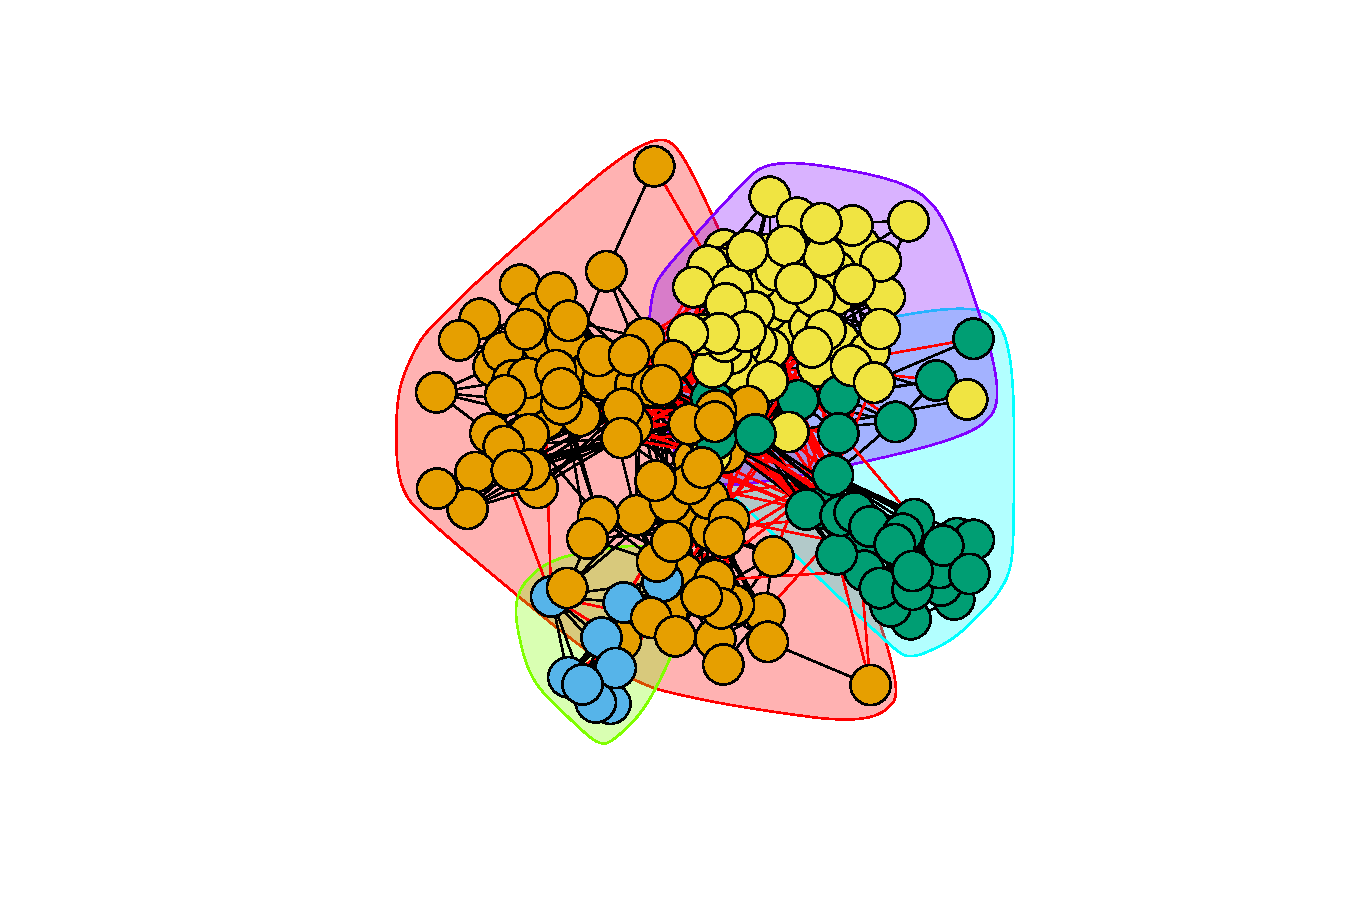
\includegraphics[width=.8\textwidth]{figures/unnamed-chunk-2-1} 
\end{knitrout}

\begin{knitrout}\scriptsize
\definecolor{shadecolor}{rgb}{0.969, 0.969, 0.969}\color{fgcolor}\begin{kframe}
\begin{alltt}
\hlstd{hc} \hlkwb{<-} \hlkwd{cluster_edge_betweenness}\hlstd{(blog)}
\hlkwd{plot}\hlstd{(hc, blog,} \hlkwc{vertex.label}\hlstd{=}\hlnum{NA}\hlstd{)}
\end{alltt}
\end{kframe}
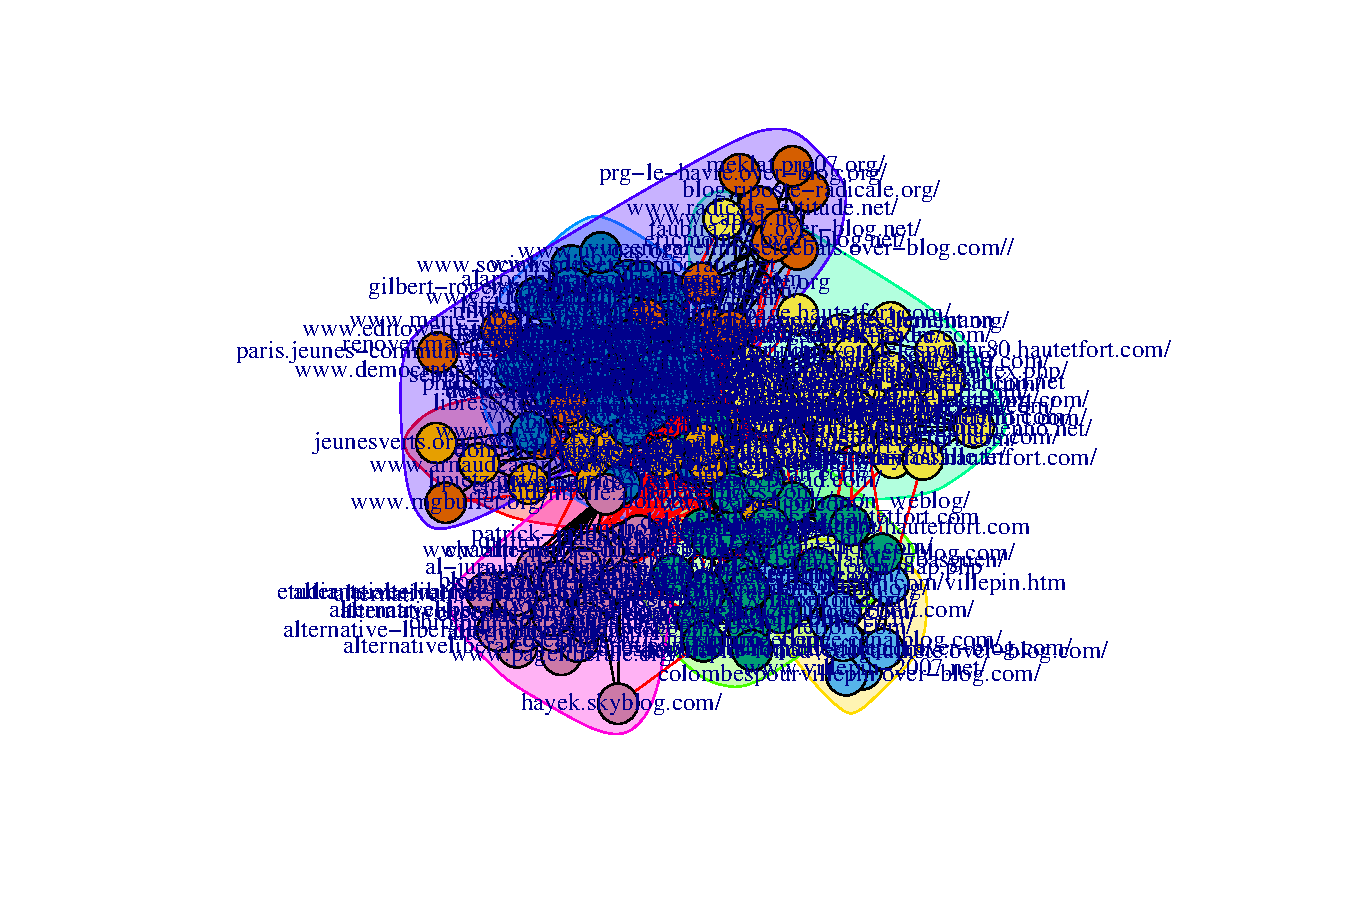
\includegraphics[width=.8\textwidth]{figures/unnamed-chunk-3-1} 
\end{knitrout}

\end{frame}

%% ==========================================================================
\subsection{Spectral methods}

\begin{frame}[fragile]
  \frametitle{Motivation: graph-cut}
  
  \begin{block}{Definition}
    The cut between two sets of nodes that form a partition in the graph is

$$
\mathrm{cut}(\mathcal{V}_A, \mathcal{V}_B) = \sum_{i\in\clV_A, j\in\clV_B} Y_{ij}, \qquad \clV_A \cup \clV_B = \clV
$$
\end{block}

\paragraph{Example:}
The graph cut between $\clV_A= \{1,2,3,4,5\}$ and $\clV_B= \{6,7,8,9,10\}$ is 2.

\begin{knitrout}\scriptsize
\definecolor{shadecolor}{rgb}{0.969, 0.969, 0.969}\color{fgcolor}
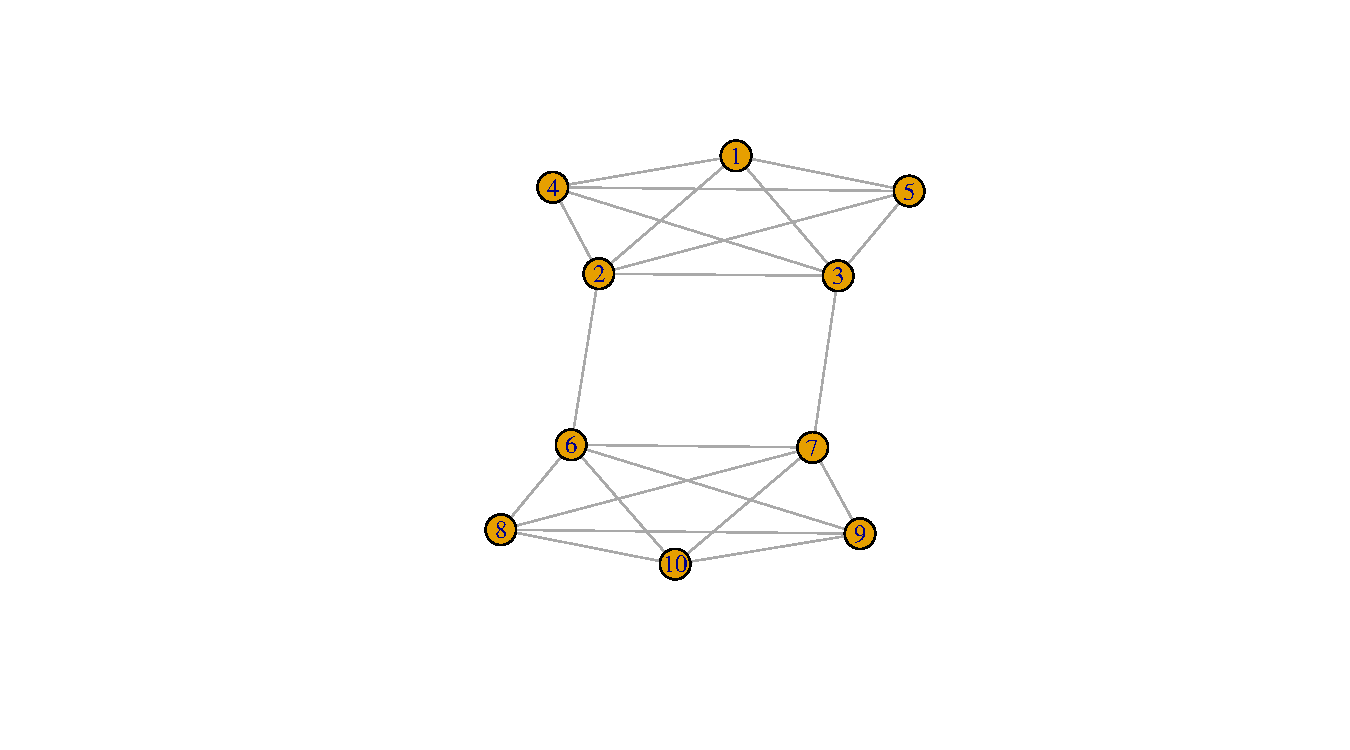
\includegraphics[width=.8\textwidth]{figures/graph-cut-plot-1} 
\end{knitrout}

\end{frame}

\begin{frame}
  \frametitle{Min-cut}
  
  \paragraph{Idea:} Find the 2-partition that minimizes the cut to form two homogeneous clusters.

  \begin{block}{Min-cut problem}
  Based on this principle, the normalized cut consider the connectivity between groups relative to the volume of each groups

$$\argmin_{\{\clV_A, \clV_B\}} \mathrm{cut}^{N}(\clV_A, \clV_B),$$

where $\mathrm{Vol}(\clV_S)) = \sum_{i\in\mathcal{S}} d_i$ and

$$
\begin{aligned}
\mathrm{cut}^{N}(\clV_A, \clV_B) & = \frac{\mathrm{cut}(\clV_A, \clV_B)}{\mathrm{Vol}(\clV_A)} + \frac{\mathrm{cut}(\clV_A, \clV_B)}{\mathrm{Vol}(\clV_B)} \\
 & =  \mathrm{cut}(\clV_A, \clV_B)\frac{\mathrm{Vol}(\clV_A) + \mathrm{Vol}(\clV_B)}{\mathrm{Vol}(\clV_A)\mathrm{Vol}(\clV_B)} \\
\end{aligned}
$$
  \end{block}
\end{frame}

\begin{frame}
  \frametitle{Solving min-cut for 2 clusters}
  
Let 

$$
x = (x_i)_{i=1,\dots,n} = 
\begin{cases}
-1 & \mathrm{if} \quad  i\in \clV_A, \\
 1 & \mathrm{if} \quad  i\in \clV_B. \\
\end{cases}
$$
Then, letting $D$ the diagonal matrix of degrees, 

$$
x^\top (D - Y) x = x^\top D x - ( x^\top D x - 2 \mathrm{cut} (\clV_A, \clV_B)),
$$

so that 

$$
\mathrm{cut} (\clV_A, \clV_B) = \frac12 x^\top (D - Y) x.
$$

\end{frame}

\begin{frame}
  \frametitle{Solving Min-cut for 2 clusters}

\begin{block}{Normalized graph-cut $\Leftrightarrow$ integer programming problem}

$$\begin{aligned}
& \argmin_{\{\clV_A, \clV_B\}}  \mathrm{cut}^{N}(\clV_A, \clV_B) \\[1.5ex]
\Leftrightarrow \quad & \argmin_{x\in\{-1, 1\}^n} \frac{x^\top (D - Y) x}{x^\top D x}, \quad \text{s.c.} \quad x^\top D \mathbf{1}_n = 0, 
\end{aligned}
$$
where the constraint imposes only discrete values in $x$. 

\end{block}

\begin{block}{Relax version}<2>
If we relax to $x\in[-1,1]^n$, it turns to a simple eigenvalue problem

$$
\argmin_{x\in[-1, 1]^n} x^\top (D - Y) x, \quad \text{s.c.} \quad x^\top D x = 1 \Leftrightarrow (D - Y) x = \lambda D x .
$$
where $\bL = D - Y$ is called the \alert{Laplacian matrix} of the graph $\mathcal{G}$.

\end{block}
  
\end{frame}

\begin{frame}[fragile]
  \frametitle{Graph Laplacian: spectrum}

  \begin{proposition}[Spectrum of $\bL$]
    The $n\times n$ matrix $\bL$ has the following properties:
    \[
      \bx^\top \bL \bx = \frac{1}{2} \sum_{i,j} Y_{ij} (x_i - x_j)^2, \quad \forall \bx\in\Rset^n .
    \]
    \vspace{-.25cm}
    \begin{itemize}
      \item $\bL$ is a symmetric, positive semi-definite matrix,
      \item $\mathbf{1}_n$ is in the kernel of $L$ since $L \mathbf{1}_n = 0$,
      \item The first normalized eigen vector with eigen value $\lambda> 0$ is solution to the relaxed graph cut problem
    \end{itemize}  
  \end{proposition}

The Laplacian is easily (and fastly) computed in \texttt{R} thanks to the \textbf{igraph} package:

\begin{knitrout}\scriptsize
\definecolor{shadecolor}{rgb}{0.969, 0.969, 0.969}\color{fgcolor}\begin{kframe}
\begin{alltt}
\hlstd{L} \hlkwb{<-} \hlkwd{laplacian_matrix}\hlstd{(blog)}
\end{alltt}
\end{kframe}
\end{knitrout}

\end{frame}

\begin{frame}[fragile]
  \frametitle{Bi-partionning and the Fiedler vector}
  
\alert{Fiedler vector} is the named sometimes given to the normalized eigen vector associated with the smallest positive eigen-value of $\bL$. 

\begin{itemize}
 \item[$\rightarrow$] solves the relaxed min-cut problem
 \item[$\rightarrow$] can be used to compute a bi-partition of a graph.
\end{itemize}

\begin{knitrout}\scriptsize
\definecolor{shadecolor}{rgb}{0.969, 0.969, 0.969}\color{fgcolor}\begin{kframe}
\begin{alltt}
\hlstd{spec_L} \hlkwb{<-} \hlkwd{eigen}\hlstd{(L); practical_zero} \hlkwb{<-} \hlnum{1e-12}
\hlstd{lambda}  \hlkwb{<-} \hlkwd{min}\hlstd{(spec_L}\hlopt{$}\hlstd{values[spec_L}\hlopt{$}\hlstd{values}\hlopt{>}\hlstd{practical_zero])}
\hlstd{fiedler} \hlkwb{<-} \hlstd{spec_L}\hlopt{$}\hlstd{vectors[,} \hlkwd{which}\hlstd{(spec_L}\hlopt{$}\hlstd{values} \hlopt{==} \hlstd{lambda)]}
\hlkwd{qplot}\hlstd{(}\hlkwc{y} \hlstd{= fiedler,} \hlkwc{colour} \hlstd{= party)} \hlopt{+} \hlstd{viridis}\hlopt{::}\hlkwd{scale_color_viridis}\hlstd{(}\hlkwc{discrete} \hlstd{=} \hlnum{TRUE}\hlstd{)}
\end{alltt}
\end{kframe}
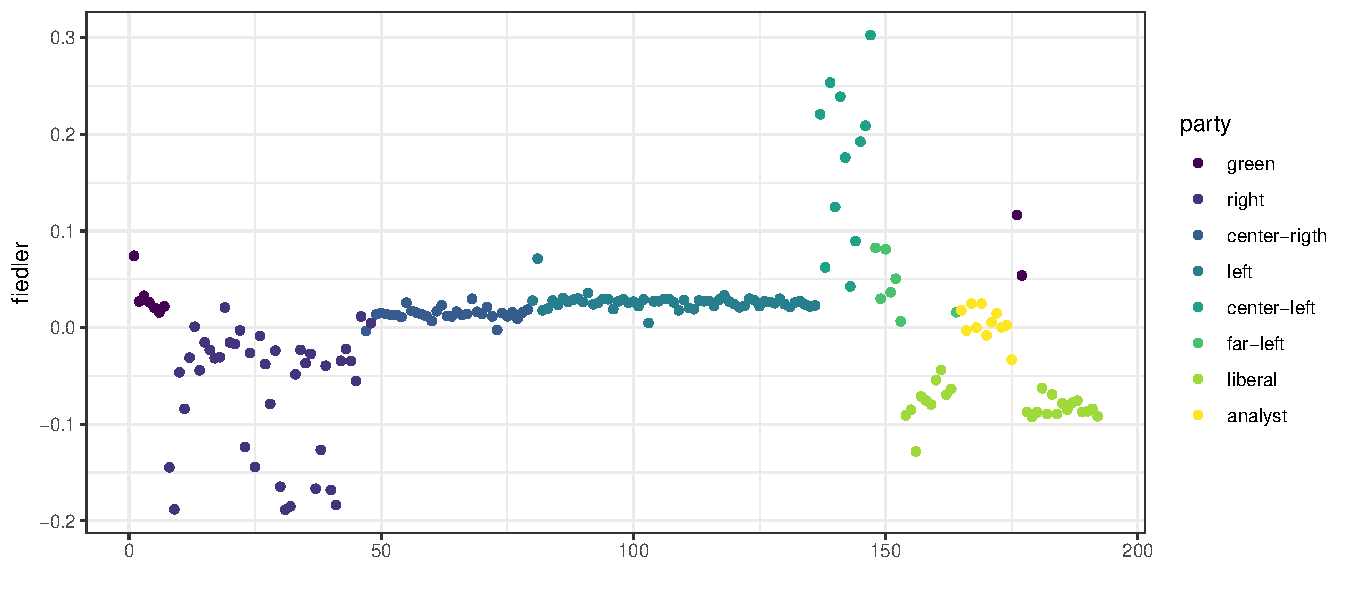
\includegraphics[width=.8\textwidth]{figures/unnamed-chunk-4-1} 
\end{knitrout}

\end{frame}

\begin{frame}[fragile]
  \frametitle{Example on a simplied left/right view}

\begin{knitrout}\scriptsize
\definecolor{shadecolor}{rgb}{0.969, 0.969, 0.969}\color{fgcolor}\begin{kframe}
\begin{alltt}
\hlstd{left_vs_right} \hlkwb{<-}
  \hlstd{forcats}\hlopt{::}\hlkwd{fct_collapse}\hlstd{(party,}
    \hlkwc{left} \hlstd{=} \hlkwd{c}\hlstd{(}\hlstr{"green"}\hlstd{,} \hlstr{"left"}\hlstd{,} \hlstr{"far-left"}\hlstd{,} \hlstr{"center-left"}\hlstd{),}
    \hlkwc{right} \hlstd{=} \hlkwd{c}\hlstd{(}\hlstr{"right"}\hlstd{,} \hlstr{"liberal"}\hlstd{,} \hlstr{"center-rigth"}\hlstd{),}
    \hlkwc{analyst} \hlstd{=} \hlstr{"analyst"}
  \hlstd{)}
\hlkwd{qplot}\hlstd{(}\hlkwc{y} \hlstd{= fiedler,} \hlkwc{colour} \hlstd{= left_vs_right)} \hlopt{+}  \hlstd{viridis}\hlopt{::}\hlkwd{scale_color_viridis}\hlstd{(}\hlkwc{discrete} \hlstd{=} \hlnum{TRUE}\hlstd{)}
\end{alltt}
\end{kframe}
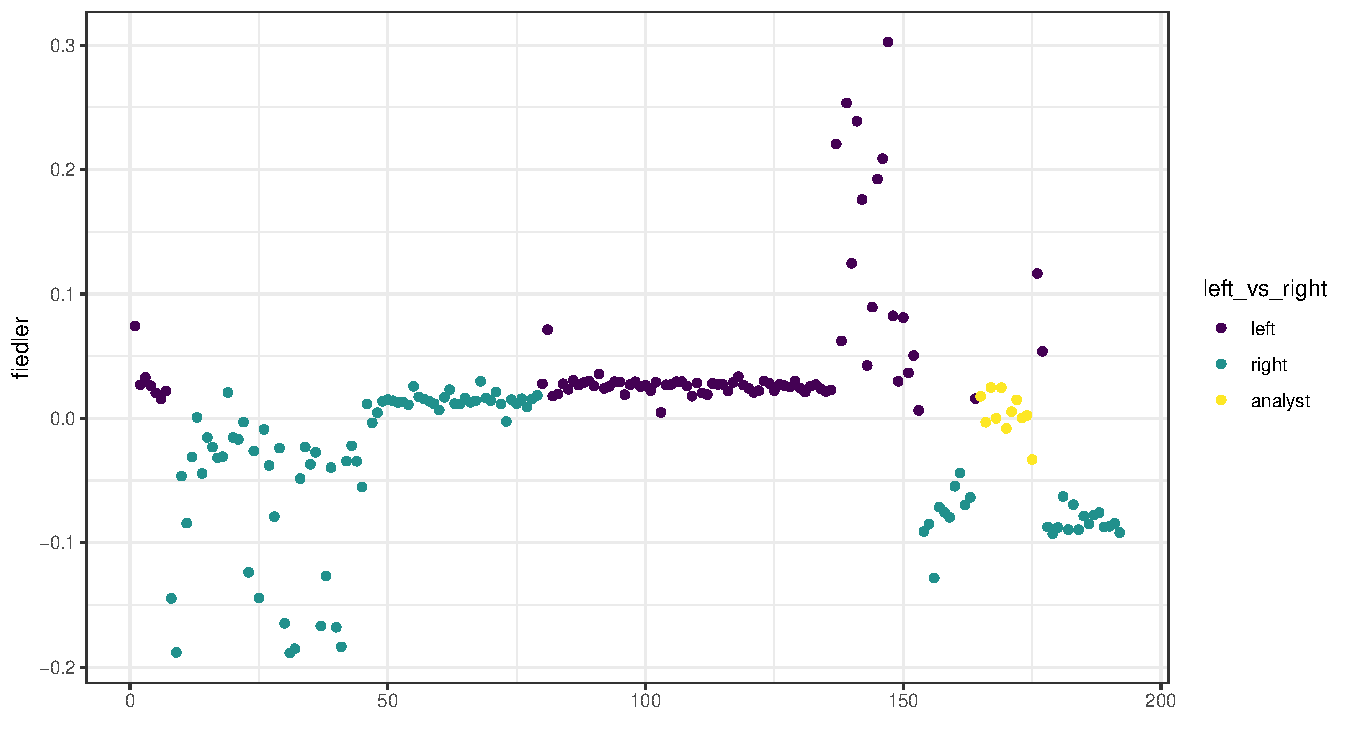
\includegraphics[width=.8\textwidth]{figures/unnamed-chunk-5-1} 
\end{knitrout}


\end{frame}

\begin{frame}[fragile]
  \frametitle{"Validation"}

\begin{knitrout}\scriptsize
\definecolor{shadecolor}{rgb}{0.969, 0.969, 0.969}\color{fgcolor}\begin{kframe}
\begin{alltt}
\hlstd{thresholds} \hlkwb{<-} \hlkwd{seq}\hlstd{(}\hlopt{-}\hlnum{.1}\hlstd{,} \hlnum{.1}\hlstd{,} \hlkwc{len} \hlstd{=} \hlnum{100}\hlstd{)}
\hlstd{ARIs} \hlkwb{<-} \hlkwd{map_dbl}\hlstd{(thresholds,} \hlopt{~}\hlkwd{ARI}\hlstd{(left_vs_right, fiedler} \hlopt{>} \hlstd{.))}
\hlkwd{qplot}\hlstd{(thresholds, ARIs)} \hlopt{+} \hlkwd{geom_vline}\hlstd{(}\hlkwc{xintercept} \hlstd{= thresholds[}\hlkwd{which.max}\hlstd{(ARIs)])} \hlopt{+} \hlkwd{theme_bw}\hlstd{()}
\end{alltt}
\end{kframe}
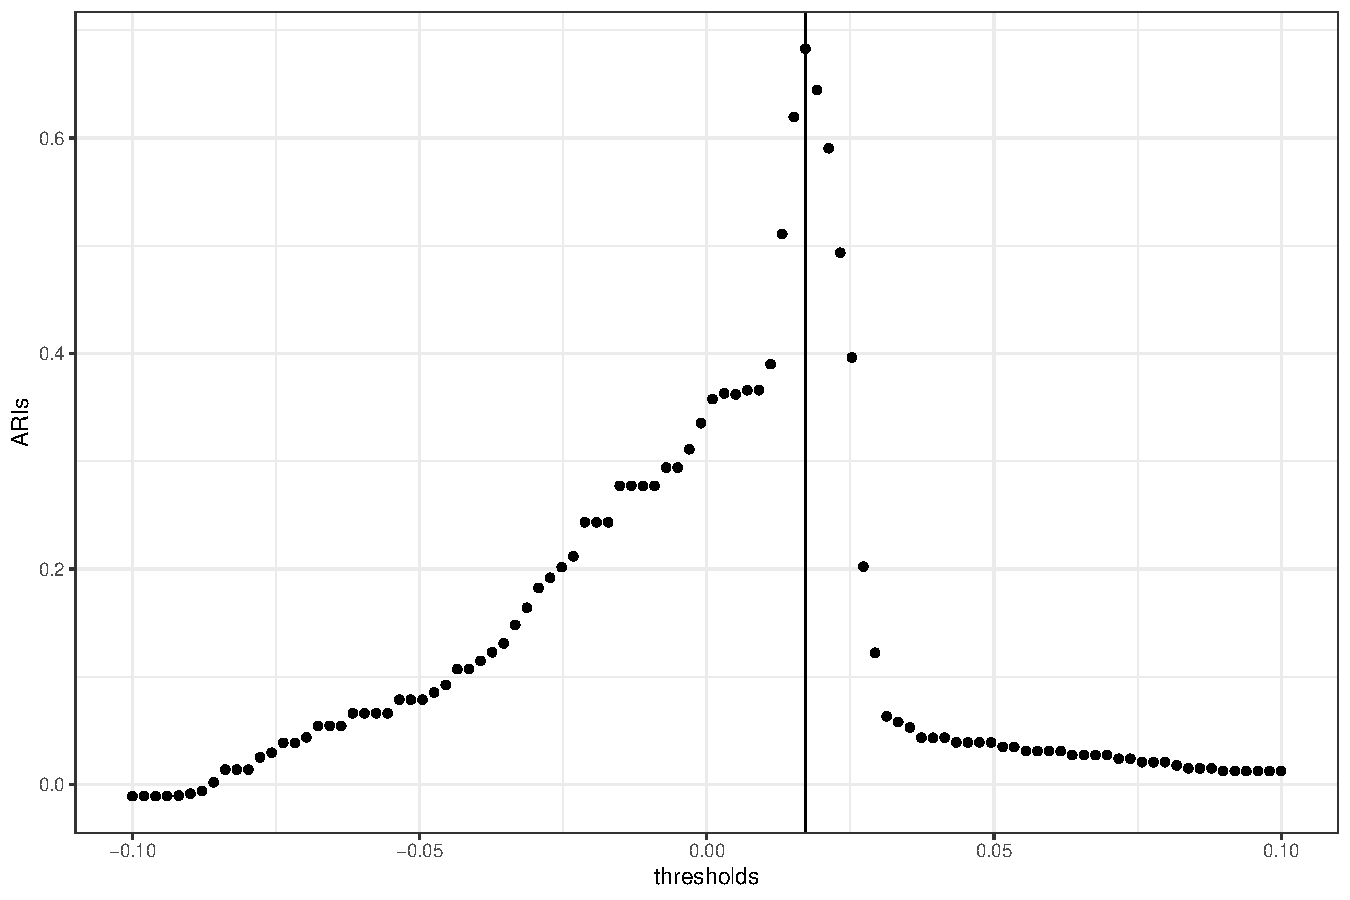
\includegraphics[width=.8\textwidth]{figures/unnamed-chunk-6-1} 
\end{knitrout}

\end{frame}

\begin{frame}
  \frametitle{Spectral clustering}

From the definition of the Laplacian matrix,
\begin{itemize}
  \item The multiplicity of the first eigen value ($0$) of $\bL$ determines the number of connected components in the graph.
  \item The larger the second non trivial (positive) eigenvalue, the higher the connectivity of $\clG$.
\end{itemize}


\begin{block}{General Heuristic}
\begin{enumerate}
\item Compute spectral decompostion of $\bL$ to perform clustering in the eigen space
\item For a graph with $K$ connected components, the first $K$ eigen-vectors are $\mathbf{1}$ spanning the eigenspace associated with eigenvalue $0$
\item Applying a simple clustering algorithm to the rows of the $K$ first eigenvectors separate the components
\end{enumerate}
\end{block}

$\rightsquigarrow$ Generalizes to graphs with a single component (tends to separates groups of nodes which are highly connected together)

\end{frame}

\begin{frame}
  \frametitle{Some variants}

  \begin{definition}[(Normalized) Laplacian]
    The normalized Laplacian matrix $\bL$ is defined by 
    \[
      \bL_N = \bD^{-1/2}\bL\bD^{-1/2} = \bI - \bD^{-1/2} \bA \bD^{-1/2}.
    \]
  \end{definition}
  
  \vfill

  \begin{definition}[(Absolute) Graph Laplacian]
    The absolute Laplacian matrix $\bL_{abs}$ is defined by 
    \[
      \bL_{abs} = \bD^{-1/2}\bA\bD^{-1/2} = \bI - \bL_N,
    \]
    with eigenvalues $1-\lambda_n \leq \dots \leq 1-\lambda_2 \leq 1-\lambda_1 = 1$, where $0=\lambda_1\leq \dots \leq \lambda_n$ are the eigenvalues of $\bL_N$.
  \end{definition}

\end{frame}

\begin{frame}
  \frametitle{Normalized Spectral Clustering}
  \framesubtitle{by Ng, Jordan and Weiss (2002)}

\begin{algorithm}[H]
  \KwIn{Adjacency matrix and number of classes $Q$}
  \BlankLine\BlankLine
  \DontPrintSemicolon
  
  Compute the normalized graph Laplacian $\mathbf{L}$\;
  Compute the eigen vectors of $\mathbf{L}$ associated with the $Q$ \alert{smallest eigenvalues}\;
  Define $\mathbf{U}$,  the $n\times Q$ matrix  that encompasses these $Q$ vectors \;
  Define $\tilde{\mathbf{U}}$, the row-wise normalized version of $\mathbf{U}$: $ \tilde{u}_{ij} = \frac{u_{ij}}{\| \mathbf{U}_i\|_2}$\;
  Apply k-means to $(\tilde{\mathbf{U}}_i)_{i=1,\dots,n}$

  \BlankLine\BlankLine
  \KwOut{vector of classes $\mathbf{C}\in \mathcal{Q}^n$, such as  $C_i = q$ if $i\in q$}

\end{algorithm}

\end{frame}

\begin{frame}[fragile]
  \frametitle{Implementation of normalized spectral clustering }

\begin{knitrout}\scriptsize
\definecolor{shadecolor}{rgb}{0.969, 0.969, 0.969}\color{fgcolor}\begin{kframe}
\begin{alltt}
\hlstd{spectral_clustering} \hlkwb{<-} \hlkwa{function}\hlstd{(}\hlkwc{graph}\hlstd{,} \hlkwc{nb_cluster}\hlstd{,} \hlkwc{normalized} \hlstd{=} \hlnum{TRUE}\hlstd{) \{}

  \hlcom{## Compute Laplacian matrix}
  \hlstd{L} \hlkwb{<-} \hlkwd{laplacian_matrix}\hlstd{(graph,} \hlkwc{normalized} \hlstd{= normalized)}
  \hlcom{## Generates indices of last (smallest) K vectors}
  \hlstd{selected} \hlkwb{<-} \hlkwd{rev}\hlstd{(}\hlnum{1}\hlopt{:}\hlkwd{ncol}\hlstd{(L))[}\hlnum{1}\hlopt{:}\hlstd{nb_cluster]}
  \hlcom{## Extract an normalized eigen-vectors}
  \hlstd{U} \hlkwb{<-} \hlkwd{eigen}\hlstd{(L)}\hlopt{$}\hlstd{vectors[, selected,} \hlkwc{drop} \hlstd{=} \hlnum{FALSE}\hlstd{]}  \hlcom{# spectral decomposition}
  \hlstd{U} \hlkwb{<-} \hlkwd{sweep}\hlstd{(U,} \hlnum{1}\hlstd{,} \hlkwd{sqrt}\hlstd{(}\hlkwd{rowSums}\hlstd{(U}\hlopt{^}\hlnum{2}\hlstd{)),} \hlstr{'/'}\hlstd{)}
  \hlcom{## Perform k-means}
  \hlstd{res} \hlkwb{<-} \hlkwd{kmeans}\hlstd{(U, nb_cluster,} \hlkwc{nstart} \hlstd{=} \hlnum{40}\hlstd{)}\hlopt{$}\hlstd{cl}

  \hlstd{res}
\hlstd{\}}
\end{alltt}
\end{kframe}
\end{knitrout}

\end{frame}

\begin{frame}[fragile]
  \frametitle{Application to the French blogosphere (1)}

Perform spectral clustering on the blogosphere for various numbers of group:

\begin{knitrout}\scriptsize
\definecolor{shadecolor}{rgb}{0.969, 0.969, 0.969}\color{fgcolor}\begin{kframe}
\begin{alltt}
\hlstd{nb_cluster} \hlkwb{<-} \hlnum{1}\hlopt{:}\hlnum{20}
\hlkwd{map}\hlstd{(nb_cluster,} \hlopt{~}\hlkwd{spectral_clustering}\hlstd{(blog, .))} \hlopt
  \hlkwd{map_dbl}\hlstd{(ARI, party)} \hlopt \hlkwd{qplot}\hlstd{(nb_cluster,} \hlkwc{y} \hlstd{= .)} \hlopt{+} \hlkwd{geom_line}\hlstd{()} \hlopt{+} \hlkwd{theme_bw}\hlstd{()}
\end{alltt}
\end{kframe}
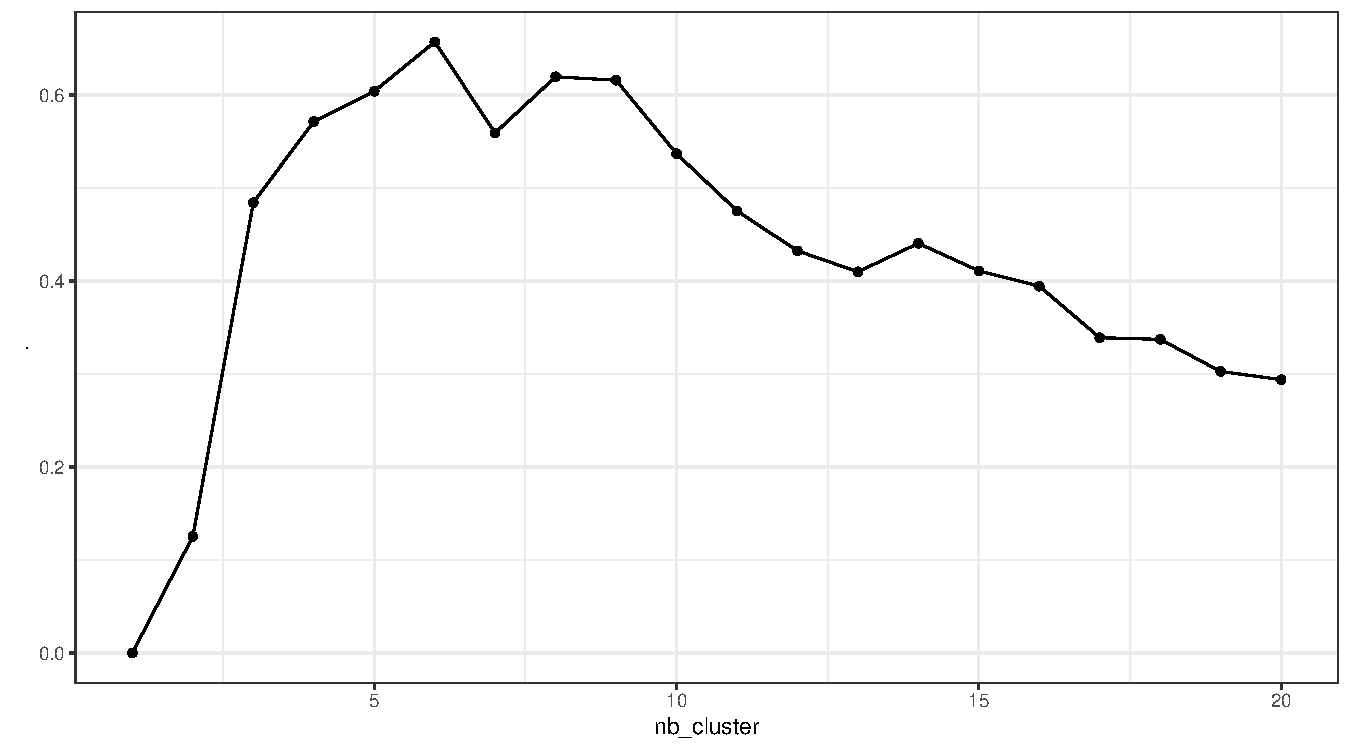
\includegraphics[width=.8\textwidth]{figures/spectral-blog-1} 
\end{knitrout}

\end{frame}

\begin{frame}[fragile]
  \frametitle{Application to the French blogosphere (2)}

Once reorder according to the best clustering (obtained $k=6$) groups, the orginal data matrix looks as follows

\begin{knitrout}\scriptsize
\definecolor{shadecolor}{rgb}{0.969, 0.969, 0.969}\color{fgcolor}\begin{kframe}
\begin{alltt}
\hlkwd{plotMyMatrix}\hlstd{(}\hlkwd{as_adj}\hlstd{(blog,} \hlkwc{sparse} \hlstd{=} \hlnum{FALSE}\hlstd{),}
  \hlkwc{clustering} \hlstd{=} \hlkwd{list}\hlstd{(}\hlkwc{row} \hlstd{=} \hlkwd{spectral_clustering}\hlstd{(blog,} \hlnum{6}\hlstd{)))}
\end{alltt}
\end{kframe}
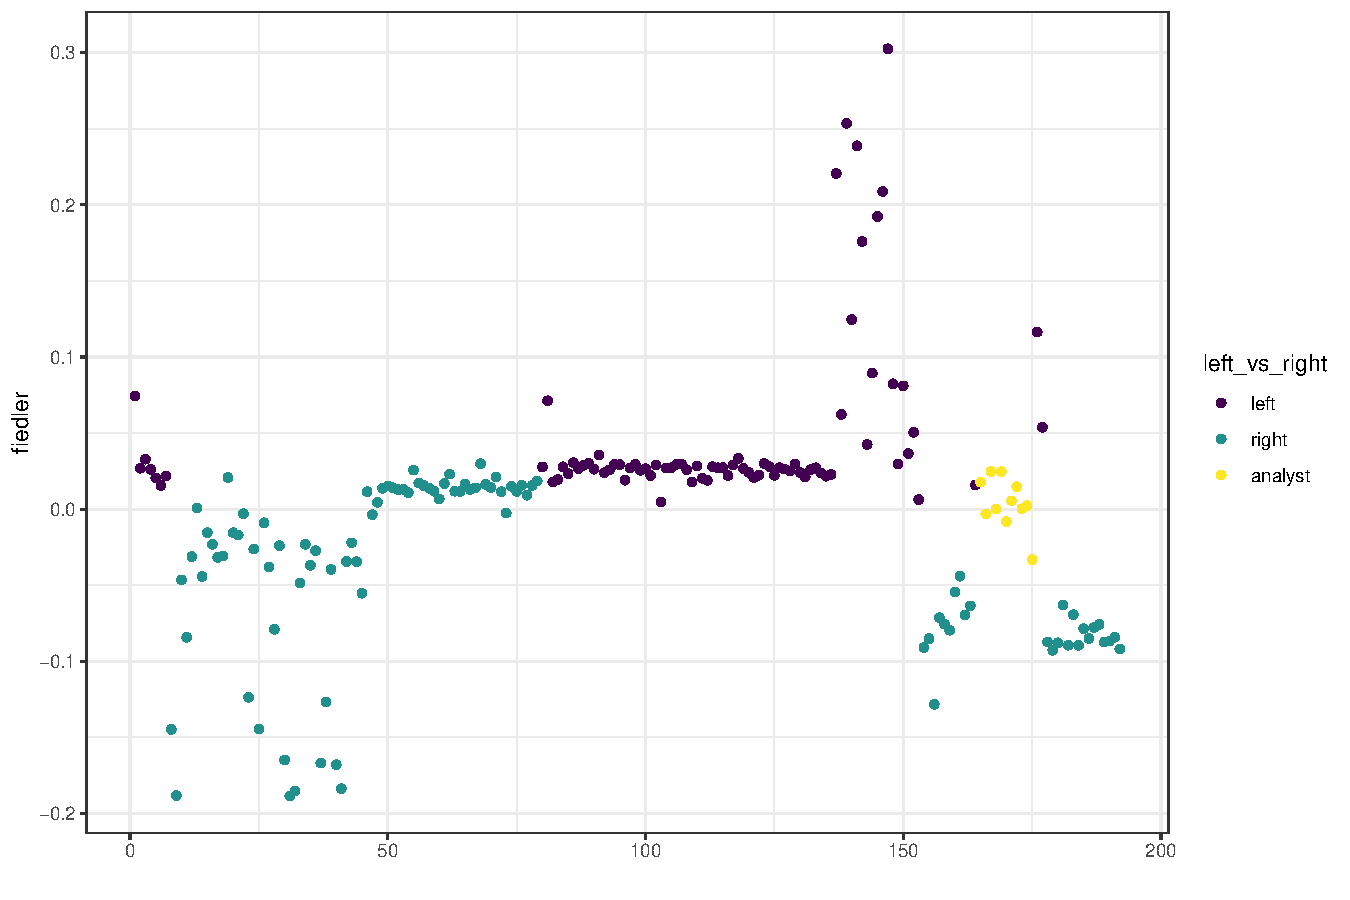
\includegraphics[width=.8\textwidth]{figures/unnamed-chunk-7-1} 
\end{knitrout}

\end{frame}

% 
% \begin{frame}
%   \frametitle{Absolute Spectral Clustering}
% 
% \begin{algorithm}[H]
%   \KwIn{Adjacency matrix and number of classes $Q$}
%   \BlankLine\BlankLine
%   \DontPrintSemicolon
% 
%   Compute the graph Laplacian $\mathbf{L}_{abs}$\;
%   Compute the eigen vectors of $\mathbf{L}_{abs}$ associated with the $Q$ \alert{largest} absolute eigenvalues\;
%   Define $\mathbf{U}$,  the $p\times Q$ matrix  that encompasses these $Q$ vectors \;
%   Apply k-means to $(\mathbf{U}_i)_{i=1,\dots,p}$
% 
%   \BlankLine\BlankLine
%   \KwOut{vector of classes $\mathbf{C}\in \mathcal{Q}^p$, such as  $C_i = q$ if $i\in q$}
% 
%   \caption{Spectral Clustering by Rohe et al. (2011)}
% \end{algorithm}
% 
% \end{frame}

%% ==========================================================================
\section{The Stochastic Block Model (SBM)}
%% ==========================================================================

\begin{frame}
  \frametitle{References}

    \begin{thebibliography}{99}
      \setbeamertemplate{bibliography item}[book]

    \bibitem[EK2]{EK2} Statistical Analysis of Network Data: Methods and Models
    \newblock \textcolor{black}{Eric Kolazcyk}
    \newblock \alert{Chapters 5 and 6}

      \setbeamertemplate{bibliography item}[article]

    \bibitem[EK2]{EK2} Mixture model for random graphs, Statistics and Computing
    \newblock \textcolor{black}{Daudin, Robin, Picard}
    \newblock {\tiny\url{pbil.univ-lyon1.fr/members/fpicard/franckpicard_fichiers/pdf/DPR08.pdf
}}

    \bibitem[CM1]{CM1} Analyse statistique de graphes,
    \newblock \textcolor{black}{Catherine Matias}
    \newblock \alert{Chapitre 4, Section 4}

    \end{thebibliography}

\end{frame}

\begin{frame}
  \frametitle{Motivations}

  \begin{block}{Last section: \alert{find an underlying organization in a observed network}}
    Spectral or hierachical clustering for network data \\
    \begin{itemize}
      \item[$\rightsquigarrow$] \alert{Not model-based}, thus no statistical inference possible
    \end{itemize}
  \end{block}

  \begin{block}{Now: \alert{clustering of network based on a probabilistic model of the graph}}
    Become familiar with
    \begin{itemize}
      \item the stochastic block model, a random graph model tailored for clustering vertices,
      \item the variational EM algorithm used to infer SBM from network data.
    \end{itemize}
  \end{block}

  \onslide{
  \begin{center}
    hierarchical/kmeans clustering $\leftrightarrow$ \alert{Gaussian mixture models} \\
      $\Updownarrow$ \\
    hierarchical/spectral clustering for network $\leftrightarrow$ Stochastic block model
  \end{center}
  }

\end{frame}

%% ==========================================================================
\subsection{Some Graphs Models and their limitations}
%% ==========================================================================

\begin{frame}
  \frametitle{A mathematical model: Erdös-Rényi graph}

  \begin{definition}
    Let $\clV = {1,\dots,n}$ be a set of fixed vertices. The (simple) Erdös-Rényi model $\mathcal{G}(n,\pi)$ assumes random edges between pairs of nodes with probability $\pi$. In orther word, the (random) adjacency matrix $\bX$ is such that
    \begin{equation*}
      X_{ij} \sim \mathcal{B}(\pi)
    \end{equation*}
  \end{definition}

  \vfill

  \begin{proposition}[degree distribution]
    The (random) degree $D_i$ of vertex $i$ follows a binomial distribution:
      \begin{equation*}
        D_i \sim b(n-1, \pi).
      \end{equation*}
  \end{proposition}

\end{frame}

\begin{frame}[fragile]
  \frametitle{Erdös-Rényi - example}

\begin{knitrout}\scriptsize
\definecolor{shadecolor}{rgb}{0.969, 0.969, 0.969}\color{fgcolor}\begin{kframe}
\begin{alltt}
\hlstd{G1} \hlkwb{<-} \hlstd{igraph}\hlopt{::}\hlkwd{sample_gnp}\hlstd{(}\hlnum{10}\hlstd{,} \hlnum{0.1}\hlstd{)}
\hlstd{G2} \hlkwb{<-} \hlstd{igraph}\hlopt{::}\hlkwd{sample_gnp}\hlstd{(}\hlnum{10}\hlstd{,} \hlnum{0.9}\hlstd{)}
\hlstd{G3} \hlkwb{<-} \hlstd{igraph}\hlopt{::}\hlkwd{sample_gnp}\hlstd{(}\hlnum{100}\hlstd{,} \hlnum{.02}\hlstd{)}
\hlkwd{par}\hlstd{(}\hlkwc{mfrow}\hlstd{=}\hlkwd{c}\hlstd{(}\hlnum{1}\hlstd{,}\hlnum{3}\hlstd{))}
\hlkwd{plot}\hlstd{(G1,} \hlkwc{vertex.label}\hlstd{=}\hlnum{NA}\hlstd{) ;} \hlkwd{plot}\hlstd{(G2,} \hlkwc{vertex.label}\hlstd{=}\hlnum{NA}\hlstd{)}
\hlkwd{plot}\hlstd{(G3,} \hlkwc{vertex.label}\hlstd{=}\hlnum{NA}\hlstd{,} \hlkwc{layout}\hlstd{=layout.circle)}
\end{alltt}
\end{kframe}
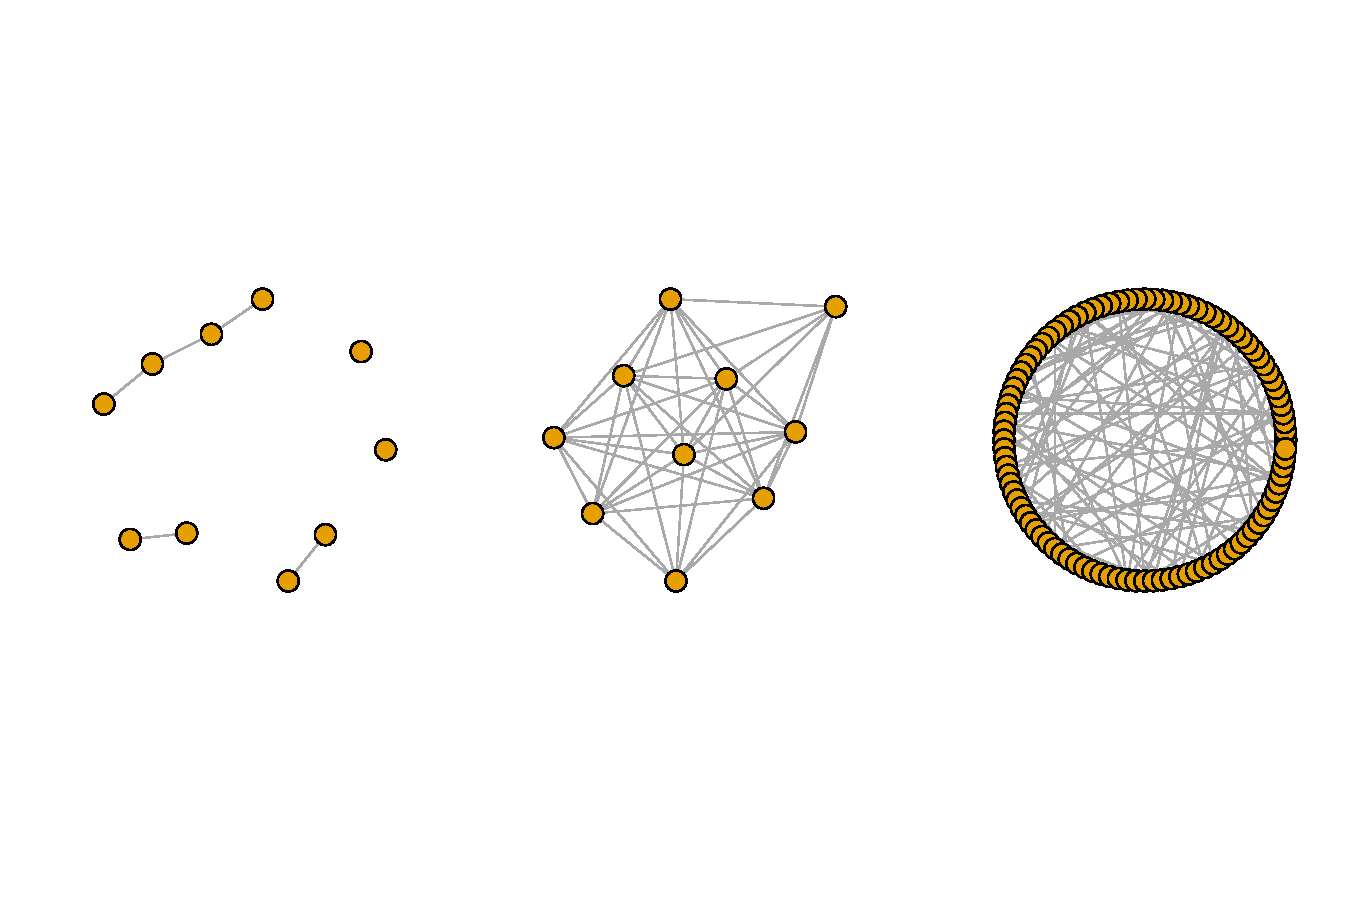
\includegraphics[width=.8\textwidth]{figures/ER_example-1} 
\end{knitrout}
\end{frame}

\begin{frame}[fragile]
  \frametitle{Erdös-Rény - limitations: very homegeneous}

\begin{knitrout}\scriptsize
\definecolor{shadecolor}{rgb}{0.969, 0.969, 0.969}\color{fgcolor}\begin{kframe}
\begin{alltt}
\hlkwd{average.path.length}\hlstd{(G3);} \hlkwd{diameter}\hlstd{(G3)}
\end{alltt}
\begin{verbatim}
## [1] 5.649385
## [1] 13
\end{verbatim}
\end{kframe}
\end{knitrout}

\begin{knitrout}\scriptsize
\definecolor{shadecolor}{rgb}{0.969, 0.969, 0.969}\color{fgcolor}
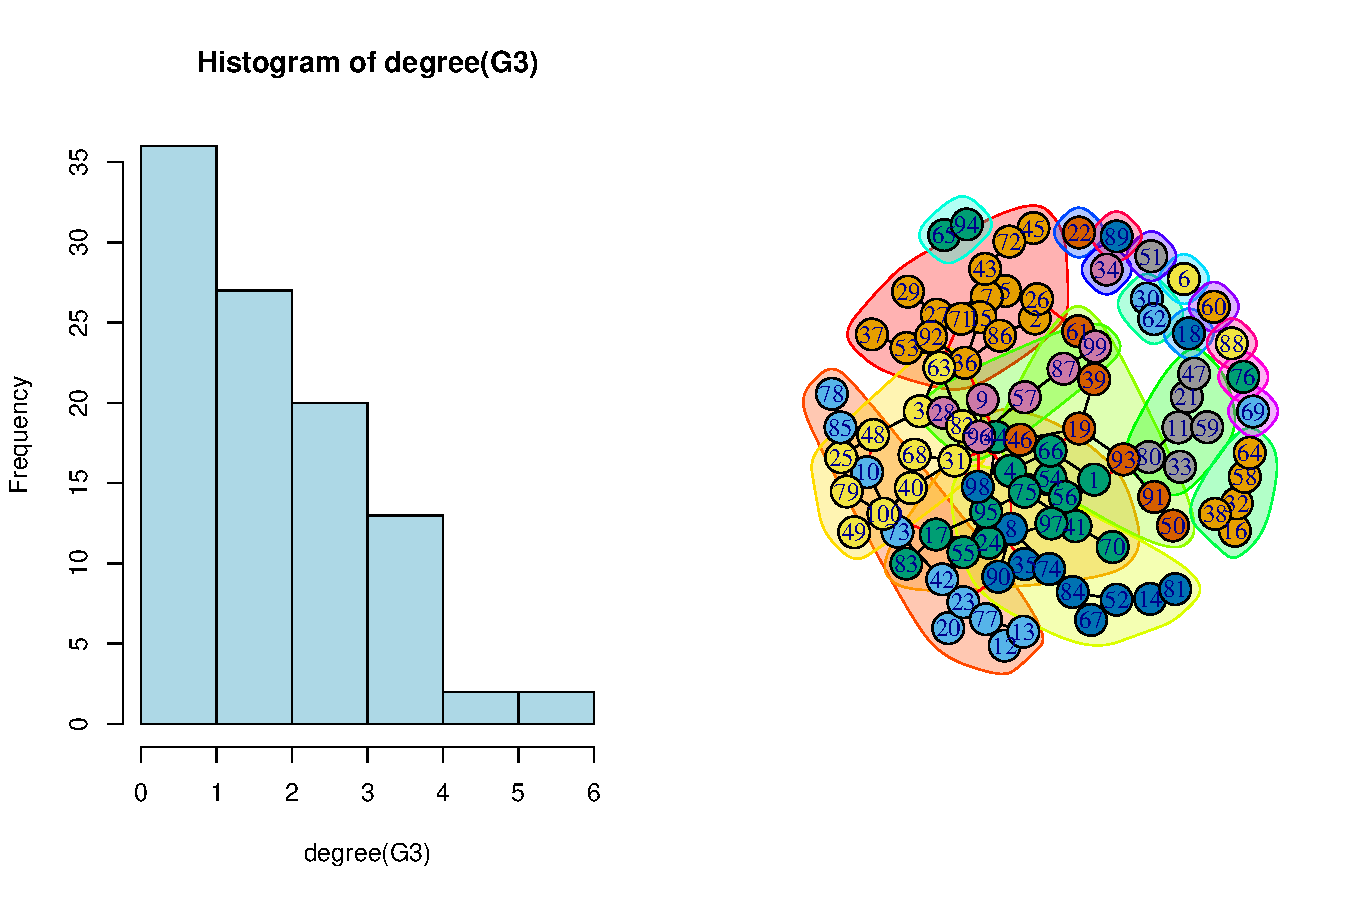
\includegraphics[width=.8\textwidth]{figures/ER_limitation2-1} 
\end{knitrout}
\end{frame}

\begin{frame}
  \frametitle{Mechanism-based model: preferential attachment}

  The graph is defined dynamically as follows
  \begin{block}{Definition}
    Start from a initial graph $\mathcal{G}_0 = (\mathcal{V}_0,\mathcal{E}_0)$, then for each time step,
    \begin{enumerate}
      \item At $t$ a new node $V_t$ is added
      \item $V_t$ is connected to $i \in V_{t-1}$ with probability
      \begin{equation*}
        D_i^\alpha + \mathrm{cst.}
      \end{equation*}
    \end{enumerate}
  \end{block}
  $\rightsquigarrow$ Nodes with high degree get more connections thus \alert{richers get richers}
\end{frame}

\begin{frame}[fragile]
  \frametitle{Preferential attachment - example}

\begin{knitrout}\scriptsize
\definecolor{shadecolor}{rgb}{0.969, 0.969, 0.969}\color{fgcolor}\begin{kframe}
\begin{alltt}
\hlstd{G1} \hlkwb{<-} \hlstd{igraph}\hlopt{::}\hlkwd{sample_pa}\hlstd{(}\hlnum{20}\hlstd{,} \hlnum{1}\hlstd{,} \hlkwc{directed}\hlstd{=}\hlnum{FALSE}\hlstd{)}
\hlstd{G2} \hlkwb{<-} \hlstd{igraph}\hlopt{::}\hlkwd{sample_pa}\hlstd{(}\hlnum{20}\hlstd{,} \hlnum{5}\hlstd{,} \hlkwc{directed}\hlstd{=}\hlnum{FALSE}\hlstd{)}
\hlstd{G3} \hlkwb{<-} \hlstd{igraph}\hlopt{::}\hlkwd{sample_pa}\hlstd{(}\hlnum{200}\hlstd{,} \hlkwc{directed}\hlstd{=}\hlnum{FALSE}\hlstd{)}
\hlkwd{par}\hlstd{(}\hlkwc{mfrow}\hlstd{=}\hlkwd{c}\hlstd{(}\hlnum{1}\hlstd{,}\hlnum{3}\hlstd{))}
\hlkwd{plot}\hlstd{(G1,} \hlkwc{vertex.label}\hlstd{=}\hlnum{NA}\hlstd{) ;} \hlkwd{plot}\hlstd{(G2,} \hlkwc{vertex.label}\hlstd{=}\hlnum{NA}\hlstd{)}
\hlkwd{plot}\hlstd{(G3,} \hlkwc{vertex.label}\hlstd{=}\hlnum{NA}\hlstd{,} \hlkwc{layout}\hlstd{=layout.circle)}
\end{alltt}
\end{kframe}
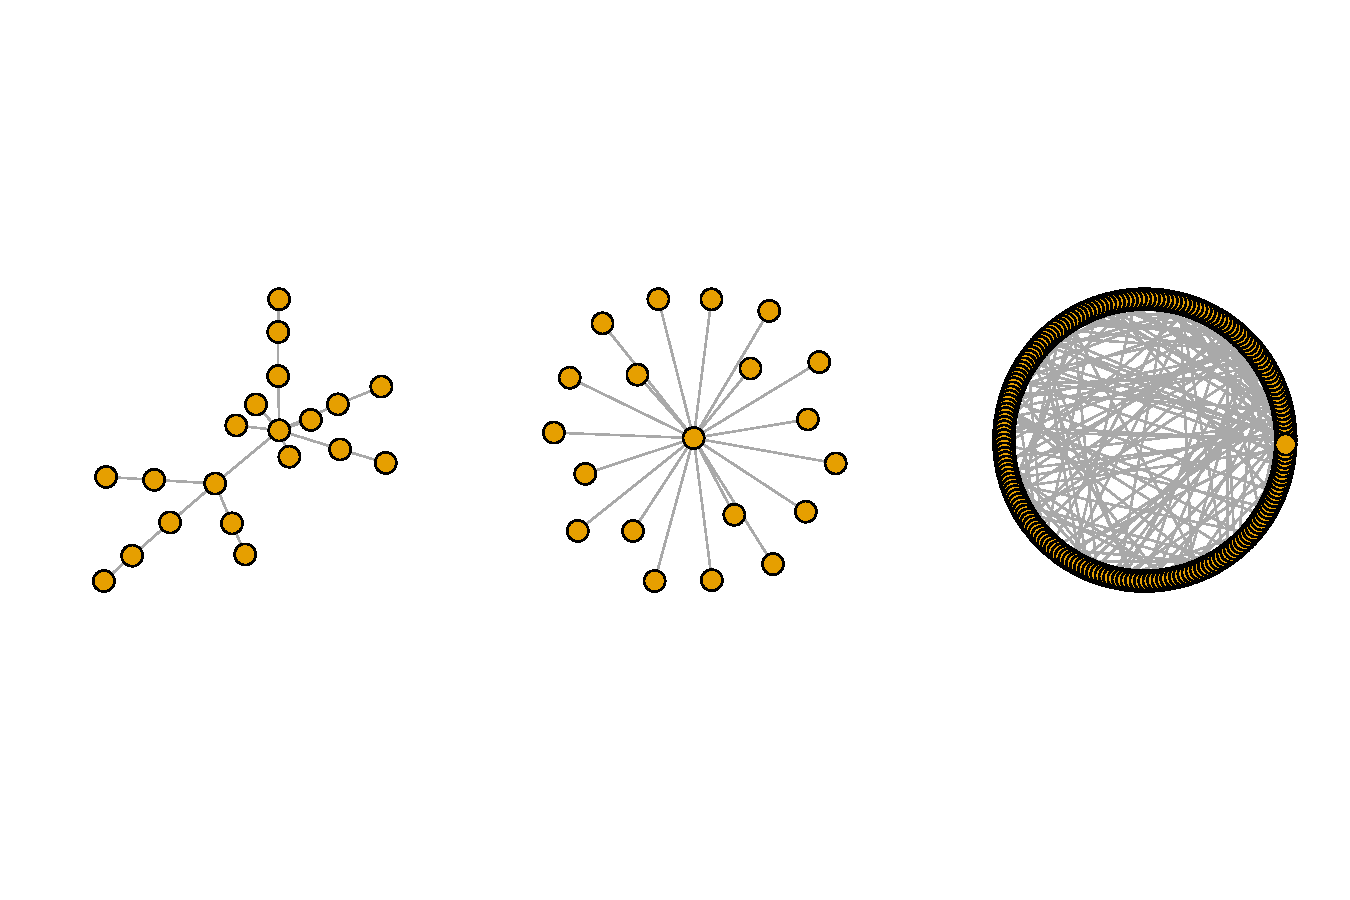
\includegraphics[width=.8\textwidth]{figures/PA_example-1} 
\end{knitrout}

\end{frame}

\begin{frame}[fragile]
  \frametitle{Preferential attachment - limitations}

\begin{knitrout}\scriptsize
\definecolor{shadecolor}{rgb}{0.969, 0.969, 0.969}\color{fgcolor}\begin{kframe}
\begin{alltt}
\hlkwd{average.path.length}\hlstd{(G3);} \hlkwd{diameter}\hlstd{(G3)}
\end{alltt}
\begin{verbatim}
## [1] 6.117387
## [1] 14
\end{verbatim}
\end{kframe}
\end{knitrout}

\begin{knitrout}\scriptsize
\definecolor{shadecolor}{rgb}{0.969, 0.969, 0.969}\color{fgcolor}
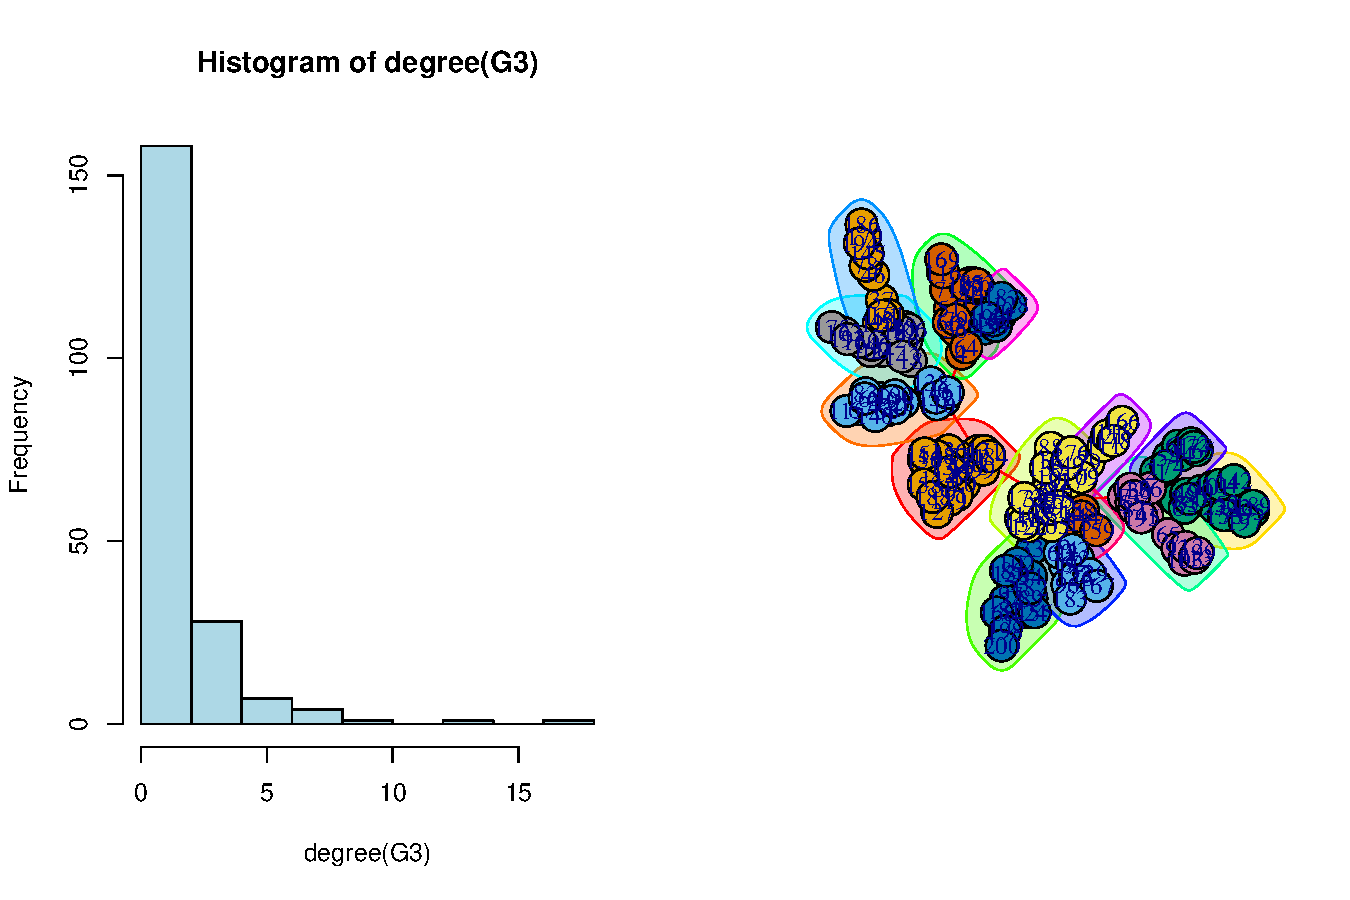
\includegraphics[width=.8\textwidth]{figures/PA_limitation2-1} 
\end{knitrout}
\end{frame}

\begin{frame}
  \frametitle{Limitations}

    \begin{itemize}
    \item \alert{Erdös-Rényi}\\
      The ER model does not fit well real world network
      \begin{itemize}
        \item As can been seen from its degree distribution
        \item ER is generally too homogeneous
      \end{itemize}
    \item \alert{Preferential attachment}
      \begin{itemize}
        \item Is defined through an algorithm so performing statistics is complicated
        \item Is stucked to the power-law distribution of degrees
      \end{itemize}
    \end{itemize}

  \vfill

  \begin{block}{The Stochastic Block Model}
    The SBM\footnote{Other models exist (e.g. exponential model for random graphs) but less popular.} generalizes ER in a mixture framework. It provides
    \begin{itemize}
      \item a statistical framework to adjust and interpret the parameters
      \item a flexible yet simple specification that fits many existing network data
    \end{itemize}
  \end{block}

\end{frame}


%% ==========================================================================
\subsection{Mixture of Erdös-Rényi and the SBM}
%% ==========================================================================

\begin{frame}
  \frametitle{Stochastic Block Model: definition}
    \framesubtitle{Mixture model point of view: mixture of Erdös-Rényi}

    \begin{block}{Latent structure}
      Let $\mathcal{V} = \set{1,..,n}$ be a fixed set of vertices. We give each $i\in\mathcal{V}$ a \alert{latent label} among a set $\mathcal{Q}=\{1,\dots,Q\}$ such that
    \begin{itemize}
    \item $\alpha_q = \prob(i\in q), \quad \sum_q \alpha_q=1$;
    \item $Z_{iq}=\1_{\{i \in  q\}}$  are independent  hidden variables.
   \end{itemize}
   \end{block}

    \begin{block}{The conditional distribution of the edges}
    Connexion probabilities depend on the node class belonging:
    \begin{equation*}
      X_{ij} | \set{i\in q, j\in\ell} \sim \mathcal{B}(\pi_{q \ell}) \qquad \bigg(\Leftrightarrow       X_{ij} | \set{Z_{iq}Z_{j\ell}=1} \sim \mathcal{B}(\pi_{q \ell}).
 \bigg)
    \end{equation*}
    The $Q\times Q$ matrix ${\boldsymbol\pi}$  gives for all couple of labels $\pi_{q\ell}=\mathbb{P}(X_{ij}=1|i\in q, j\in\ell)$.
   \end{block}

\end{frame}


\begin{frame}
  \frametitle{Stochastic Block Model: the big picture}

  \begin{center}
    \begin{overlayarea}{\textwidth}{.5\textheight}
      \begin{columns}
        \begin{column}{.45\paperwidth}
        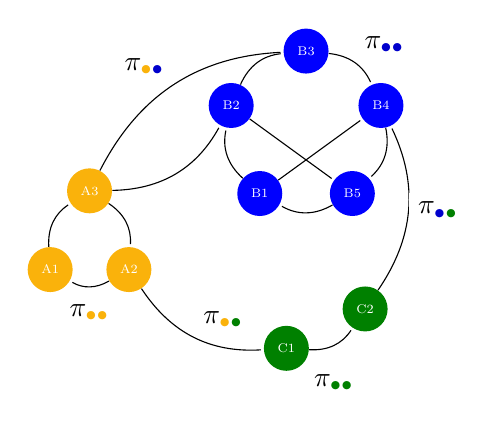
\begin{tikzpicture}
          %% UN GRAPH

          \tikzstyle{every edge}=[-,>=stealth',shorten >=1pt,auto,thin,draw]
          \tikzstyle{every state}=[draw=none,text=white,scale=0.65, font=\scriptsize, transform shape]
          \tikzstyle{every node}=[fill=yellow!40!orange]
          % premier cluster
          \node[state] (A1) at (0,0.5) {A1};
          \node[state] (A2) at (1,0.5) {A2};
          \node[state] (A3) at (.5,1.5) {A3};

          \path (A2) edge [bend left] node[fill=white,below=.1cm]
          {$\pi_{\textcolor{yellow!40!orange}{\bullet}\textcolor{yellow!40!orange}{\bullet}}$}
          (A1)
          (A1) edge [bend left] (A3)
          (A3) edge [bend left] (A2);

          \tikzstyle{every node}=[fill=blue!80!black]
          \foreach \angle/\text in {234/B1, 162/B2, 90/B3, 18/B4, -54/B5} {
            \node[fill=blue,state,xshift=5cm,yshift=3.5cm]     (\text)    at
            (\angle:1cm) {\text};
          }
          \path (B2) edge (B5)
          (B1) edge (B4);
          \foreach \from/\to in {1/2,2/3,4/5,5/1}{
            \path (B\from) edge [bend left] (B\to);
          }

          \path    (B3)    edge     [bend    left]    node[fill=white]
          {$\pi_{\textcolor{blue!80!black}{\bullet}\textcolor{blue!80!black}{\bullet}}$}  (B4) ;

          \tikzstyle{every node}=[fill=green!50!black]
          % troisieme cluster
          \node[state] (C1) at (3,-.5) {C1};
          \node[state] (C2) at (4,0) {C2};

          \path (C1) edge [bend right] node[fill=white,below=.25cm]
          {$\pi_{\textcolor{green!50!black}{\bullet}\textcolor{green!50!black}{\bullet}}$}
          (C2);

          % inter cluster
          \path (A3) edge [bend right]  (B2)
          (A3)    edge    [bend    left]    node[fill=white]
          {$\pi_{\textcolor{yellow!40!orange}{\bullet}\textcolor{blue!80!black}{\bullet}}$}
          (B3)
          (C2) edge [bend right] node[fill=white,right]
          {$\pi_{\textcolor{blue!80!black}{\bullet}\textcolor{green!50!black}{\bullet}}$}
          (B4)
          (A2) edge [bend right] node[fill=white]
          {$\pi_{\textcolor{yellow!40!orange}{\bullet}\textcolor{green!50!black}{\bullet}}$}
          (C1);
        \end{tikzpicture}
        \end{column}
        \begin{column}{.5\paperwidth}
          \begin{small}
            \begin{block}{Stochastic Block Model}
              Let $n$ nodes divided into
              \begin{itemize}
              \item
                $\mathcal{Q}=\{\textcolor{yellow!40!orange}{\bullet},\textcolor{blue!80!black}{\bullet},\textcolor{green!50!black}{\bullet}\}$
                classes
              \item  $\alpha_\bullet  =  \mathbb{P}(i  \in  \bullet)$,
                $\bullet\in\mathcal{Q},i=1,\dots,n$
              \item      $\pi_{\textcolor{yellow!40!orange}{\bullet}\textcolor{blue!80!black}{\bullet}}     =      \mathbb{P}(i
                \leftrightarrow j | i\in\textcolor{yellow!40!orange}{\bullet},j\in\textcolor{blue!80!black}{\bullet})$
              \end{itemize}
            \end{block}
          \end{small}
        \end{column}
      \end{columns}
    \end{overlayarea}
  \end{center}

  \begin{align*}
    Z_i = \mathbf{1}_{\{i \in \bullet\}}  \ & \sim^{\text{iid}} \mathcal{M}(1,\alpha), \quad \forall\bullet\in\mathcal{Q}, \\
    X_{ij} \ | \ \{i\in\textcolor{yellow!40!orange}{\bullet},j\in\textcolor{blue!80!black}{\bullet}\} & \sim^{\text{ind}} \mathcal{B}(\pi_{\textcolor{yellow!40!orange}{\bullet}\textcolor{blue!80!black}{\bullet}})\\
  \end{align*}

\end{frame}

\begin{frame}
  \frametitle{Stochastic Block Model: unknown parameters}

    \begin{center}
  \begin{overlayarea}{\textwidth}{.5\textheight}
      \begin{columns}
        \begin{column}{.45\paperwidth}
        \begin{tikzpicture}
          %% UN GRAPH

          \tikzstyle{every edge}=[-,>=stealth',shorten >=1pt,auto,thin,draw]
          \tikzstyle{every state}=[draw=none,text=white,scale=0.65, font=\scriptsize, transform shape]
          \tikzstyle{every node}=[fill=gray]
          % premier cluster
          \node[state] (A1) at (0,0.5) {N1};
          \node[state] (A2) at (1,0.5) {N2};
          \node[state] (A3) at (.5,1.5) {N3};

          \path (A2) edge [bend left] node[fill=white,below=.1cm]
          {}
          (A1)
          (A1) edge [bend left] (A3)
          (A3) edge [bend left] (A2);

          \tikzstyle{every node}=[fill=blue!80!black]
          \foreach \angle/\text in {234/N1, 162/N2, 90/N3, 18/N4, -54/N5} {
            \node[fill=gray,state,xshift=5cm,yshift=3.5cm]     (\text)    at
            (\angle:1cm) {\text};
          }
          \path (B2) edge (B5)
          (B1) edge (B4);
          \foreach \from/\to in {1/2,2/3,4/5,5/1}{
            \path (B\from) edge [bend left] (B\to);
          }

          \path (B3) edge [bend left] node[fill=white] {}  (B4) ;

          \tikzstyle{every node}=[fill=gray]
          % troisime cluster
          \node[state] (C1) at (3,-.5) {N1};
          \node[state] (C2) at (4,0) {N2};

          \path (C1) edge [bend right] (C2);

          % inter cluster
          \path (A3) edge [bend right]  (B2)
          (A3)    edge    [bend    left]    node[fill=white]
          {}
          (B3)
          (C2) edge [bend right] node[fill=white,right]
          {}
          (B4)
          (A2) edge [bend right] node[fill=white]
          {}
          (C1);
        \end{tikzpicture}
        \end{column}
        \begin{column}{.5\paperwidth}
          \begin{small}
            \begin{block}{Stochastic Block Model}
              Let $n$ nodes divided into
              \begin{itemize}
              \item
                $\mathcal{Q}=\{\textcolor{yellow!40!orange}{\bullet},\textcolor{blue!80!black}{\bullet},\textcolor{green!50!black}{\bullet}\}$,
                $\text{card}(\mathcal{Q})$ known
              \item  $\alpha_\bullet  =  ?$,
              \item      $\pi_{\textcolor{yellow!40!orange}{\bullet}\textcolor{blue!80!black}{\bullet}}     =      ?$
              \end{itemize}
            \end{block}
          \end{small}
        \end{column}
      \end{columns}
    \end{overlayarea}
    \end{center}

  \begin{align*}
    Z_i = \mathbf{1}_{\{i \in \bullet\}}  \ & \sim^{\text{iid}} \mathcal{M}(1,\alpha), \quad \forall\bullet\in\mathcal{Q}, \\
    X_{ij} \ | \ \{i\in\textcolor{yellow!40!orange}{\bullet},j\in\textcolor{blue!80!black}{\bullet}\} & \sim^{\text{ind}} \mathcal{B}(\pi_{\textcolor{yellow!40!orange}{\bullet}\textcolor{blue!80!black}{\bullet}})\\
  \end{align*}

\end{frame}

\begin{frame}[fragile]
  \frametitle{Stochastic block models -- examples of topology}
  \framesubtitle{Community network}

\begin{knitrout}\scriptsize
\definecolor{shadecolor}{rgb}{0.969, 0.969, 0.969}\color{fgcolor}\begin{kframe}
\begin{alltt}
\hlstd{pi} \hlkwb{<-} \hlkwd{matrix}\hlstd{(}\hlkwd{c}\hlstd{(}\hlnum{0.3}\hlstd{,}\hlnum{0.02}\hlstd{,}\hlnum{0.02}\hlstd{,}\hlnum{0.02}\hlstd{,}\hlnum{0.3}\hlstd{,}\hlnum{0.02}\hlstd{,}\hlnum{0.02}\hlstd{,}\hlnum{0.02}\hlstd{,}\hlnum{0.3}\hlstd{),}\hlnum{3}\hlstd{,}\hlnum{3}\hlstd{)}
\hlstd{communities} \hlkwb{<-} \hlstd{igraph}\hlopt{::}\hlkwd{sample_sbm}\hlstd{(}\hlnum{100}\hlstd{, pi,} \hlkwd{c}\hlstd{(}\hlnum{25}\hlstd{,} \hlnum{50}\hlstd{,} \hlnum{25}\hlstd{))}
\hlkwd{par}\hlstd{(}\hlkwc{mfrow} \hlstd{=} \hlkwd{c}\hlstd{(}\hlnum{1}\hlstd{,}\hlnum{2}\hlstd{))}
\hlkwd{plot}\hlstd{(communities,} \hlkwc{vertex.label}\hlstd{=}\hlnum{NA}\hlstd{,} \hlkwc{vertex.color} \hlstd{=} \hlkwd{rep}\hlstd{(}\hlnum{1}\hlopt{:}\hlnum{3}\hlstd{,}\hlkwd{c}\hlstd{(}\hlnum{25}\hlstd{,} \hlnum{50}\hlstd{,} \hlnum{25}\hlstd{)))}
\hlkwd{corrplot}\hlstd{(}\hlkwd{as_adj}\hlstd{(communities,} \hlkwc{sparse} \hlstd{=}\hlnum{FALSE}\hlstd{),} \hlkwc{tl.pos} \hlstd{=} \hlstr{"n"}\hlstd{,} \hlkwc{cl.pos} \hlstd{=} \hlstr{'n'}\hlstd{)}
\end{alltt}
\end{kframe}
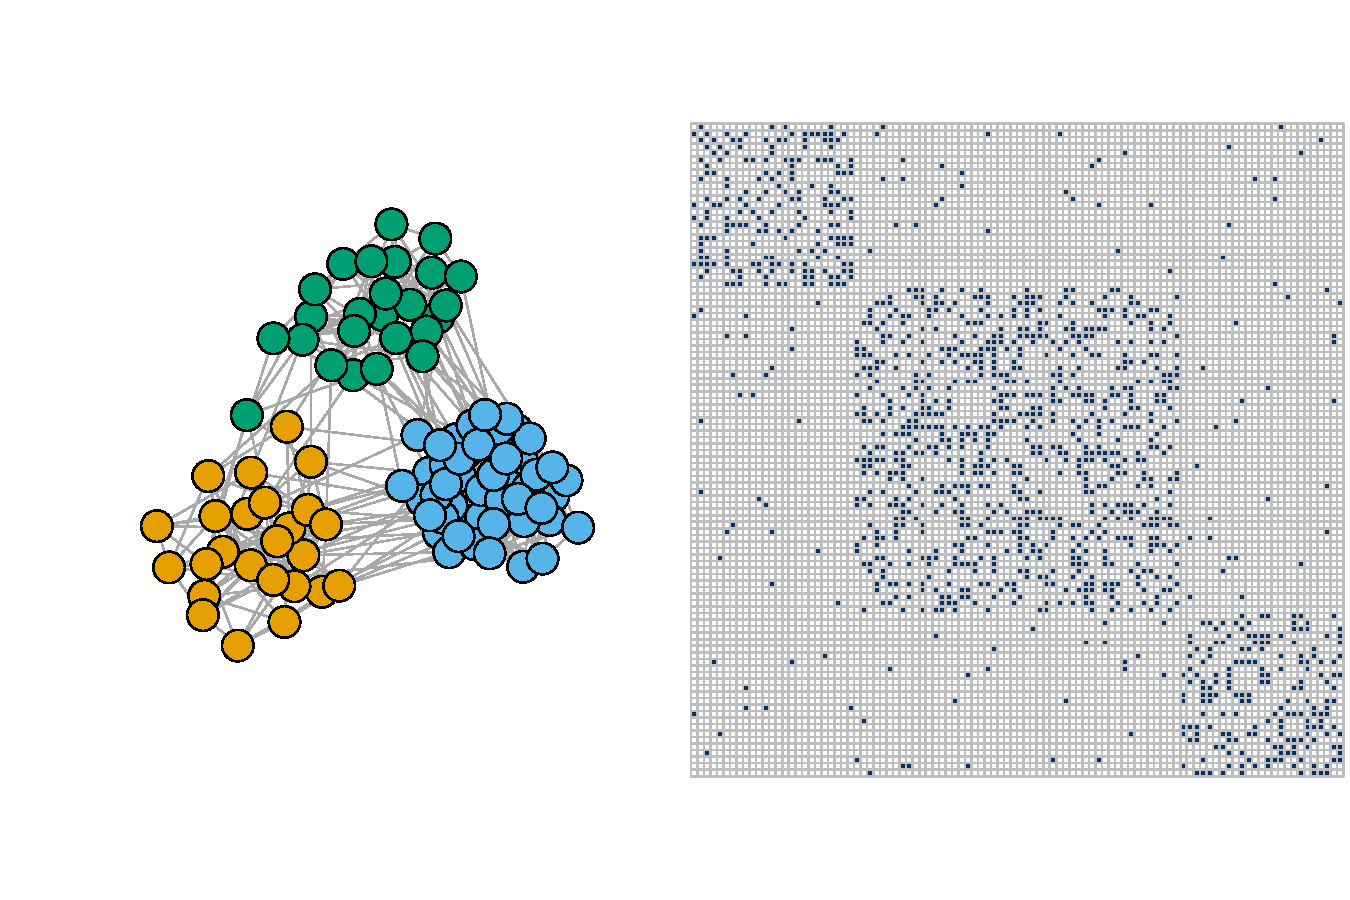
\includegraphics[width=.8\textwidth]{figures/unnamed-chunk-8-1} 
\end{knitrout}

\end{frame}

\begin{frame}[fragile]
  \frametitle{Stochastic block models -- examples of topology}
  \framesubtitle{Star network}

\begin{knitrout}\scriptsize
\definecolor{shadecolor}{rgb}{0.969, 0.969, 0.969}\color{fgcolor}\begin{kframe}
\begin{alltt}
\hlstd{pi} \hlkwb{<-} \hlkwd{matrix}\hlstd{(}\hlkwd{c}\hlstd{(}\hlnum{0.05}\hlstd{,}\hlnum{0.3}\hlstd{,}\hlnum{0.3}\hlstd{,}\hlnum{0}\hlstd{),}\hlnum{2}\hlstd{,}\hlnum{2}\hlstd{)}
\hlstd{star} \hlkwb{<-} \hlstd{igraph}\hlopt{::}\hlkwd{sample_sbm}\hlstd{(}\hlnum{100}\hlstd{, pi,} \hlkwd{c}\hlstd{(}\hlnum{4}\hlstd{,} \hlnum{96}\hlstd{))}
\hlkwd{par}\hlstd{(}\hlkwc{mfrow} \hlstd{=} \hlkwd{c}\hlstd{(}\hlnum{1}\hlstd{,}\hlnum{2}\hlstd{))}
\hlkwd{plot}\hlstd{(star,} \hlkwc{vertex.label}\hlstd{=}\hlnum{NA}\hlstd{,} \hlkwc{vertex.color} \hlstd{=} \hlkwd{rep}\hlstd{(}\hlnum{1}\hlopt{:}\hlnum{2}\hlstd{,}\hlkwd{c}\hlstd{(}\hlnum{4}\hlstd{,}\hlnum{96}\hlstd{)))}
\hlkwd{corrplot}\hlstd{(}\hlkwd{as_adj}\hlstd{(star,} \hlkwc{sparse} \hlstd{=}\hlnum{FALSE}\hlstd{),} \hlkwc{tl.pos} \hlstd{=} \hlstr{"n"}\hlstd{,} \hlkwc{cl.pos} \hlstd{=} \hlstr{'n'}\hlstd{)}
\end{alltt}
\end{kframe}
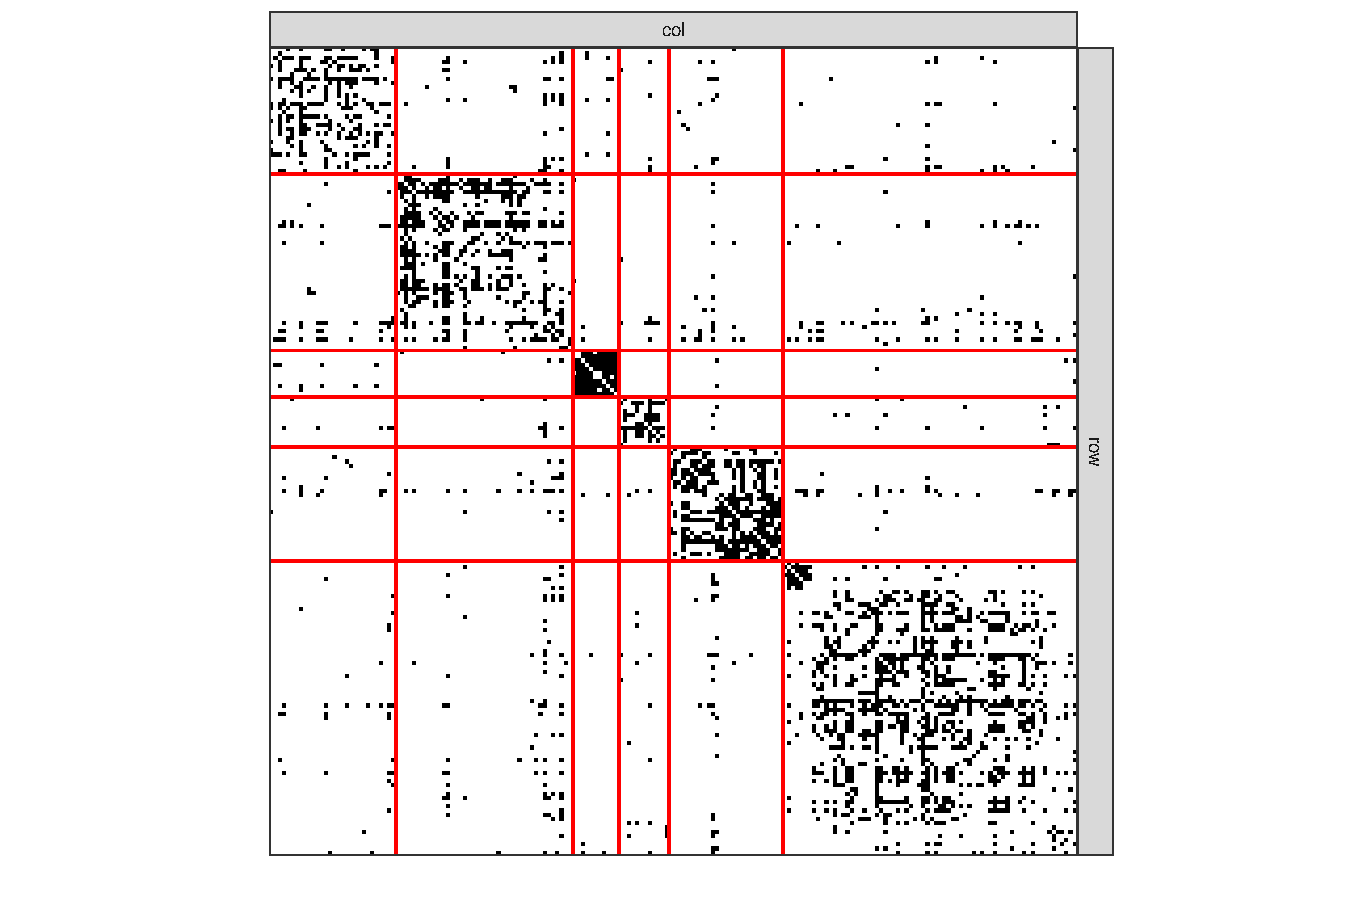
\includegraphics[width=.8\textwidth]{figures/unnamed-chunk-9-1} 
\end{knitrout}

\end{frame}

\begin{frame}[fragile]
  \frametitle{Stochastic block models -- examples of topology}
  \framesubtitle{Bipartite network}

\begin{knitrout}\scriptsize
\definecolor{shadecolor}{rgb}{0.969, 0.969, 0.969}\color{fgcolor}\begin{kframe}
\begin{alltt}
\hlstd{pi} \hlkwb{<-} \hlkwd{matrix}\hlstd{(}\hlkwd{c}\hlstd{(}\hlnum{.2}\hlstd{,}\hlnum{1}\hlopt{-}\hlnum{.2}\hlstd{,}\hlnum{.2}\hlstd{,}\hlnum{.2}\hlstd{,}\hlnum{1}\hlopt{-}\hlnum{.2}\hlstd{,}\hlnum{.2}\hlstd{,}\hlnum{.2}\hlstd{,}\hlnum{.2}\hlstd{,}\hlnum{.2}\hlstd{,}\hlnum{.2}\hlstd{,} \hlnum{.2}\hlstd{,}\hlnum{1}\hlopt{-}\hlnum{.2}\hlstd{,}\hlnum{.2}\hlstd{,}\hlnum{.2}\hlstd{,}\hlnum{1}\hlopt{-}\hlnum{.2}\hlstd{,}\hlnum{.2}\hlstd{),}\hlnum{4}\hlstd{,}\hlnum{4}\hlstd{)}
\hlstd{bipar} \hlkwb{<-} \hlstd{igraph}\hlopt{::}\hlkwd{sample_sbm}\hlstd{(}\hlnum{100}\hlstd{, pi,} \hlkwd{c}\hlstd{(}\hlnum{15}\hlstd{,} \hlnum{35}\hlstd{,} \hlnum{5}\hlstd{,} \hlnum{45}\hlstd{))}
\hlkwd{par}\hlstd{(}\hlkwc{mfrow} \hlstd{=} \hlkwd{c}\hlstd{(}\hlnum{1}\hlstd{,}\hlnum{2}\hlstd{))}
\hlkwd{plot}\hlstd{(bipar,} \hlkwc{vertex.label}\hlstd{=}\hlnum{NA}\hlstd{,} \hlkwc{vertex.color} \hlstd{=} \hlkwd{rep}\hlstd{(}\hlnum{1}\hlopt{:}\hlnum{4}\hlstd{,}\hlkwd{c}\hlstd{(}\hlnum{15}\hlstd{,} \hlnum{35}\hlstd{,} \hlnum{5}\hlstd{,} \hlnum{45}\hlstd{)))}
\hlkwd{corrplot}\hlstd{(}\hlkwd{as_adj}\hlstd{(bipar,} \hlkwc{sparse} \hlstd{=}\hlnum{FALSE}\hlstd{),} \hlkwc{tl.pos} \hlstd{=} \hlstr{"n"}\hlstd{,} \hlkwc{cl.pos} \hlstd{=} \hlstr{'n'}\hlstd{)}
\end{alltt}
\end{kframe}
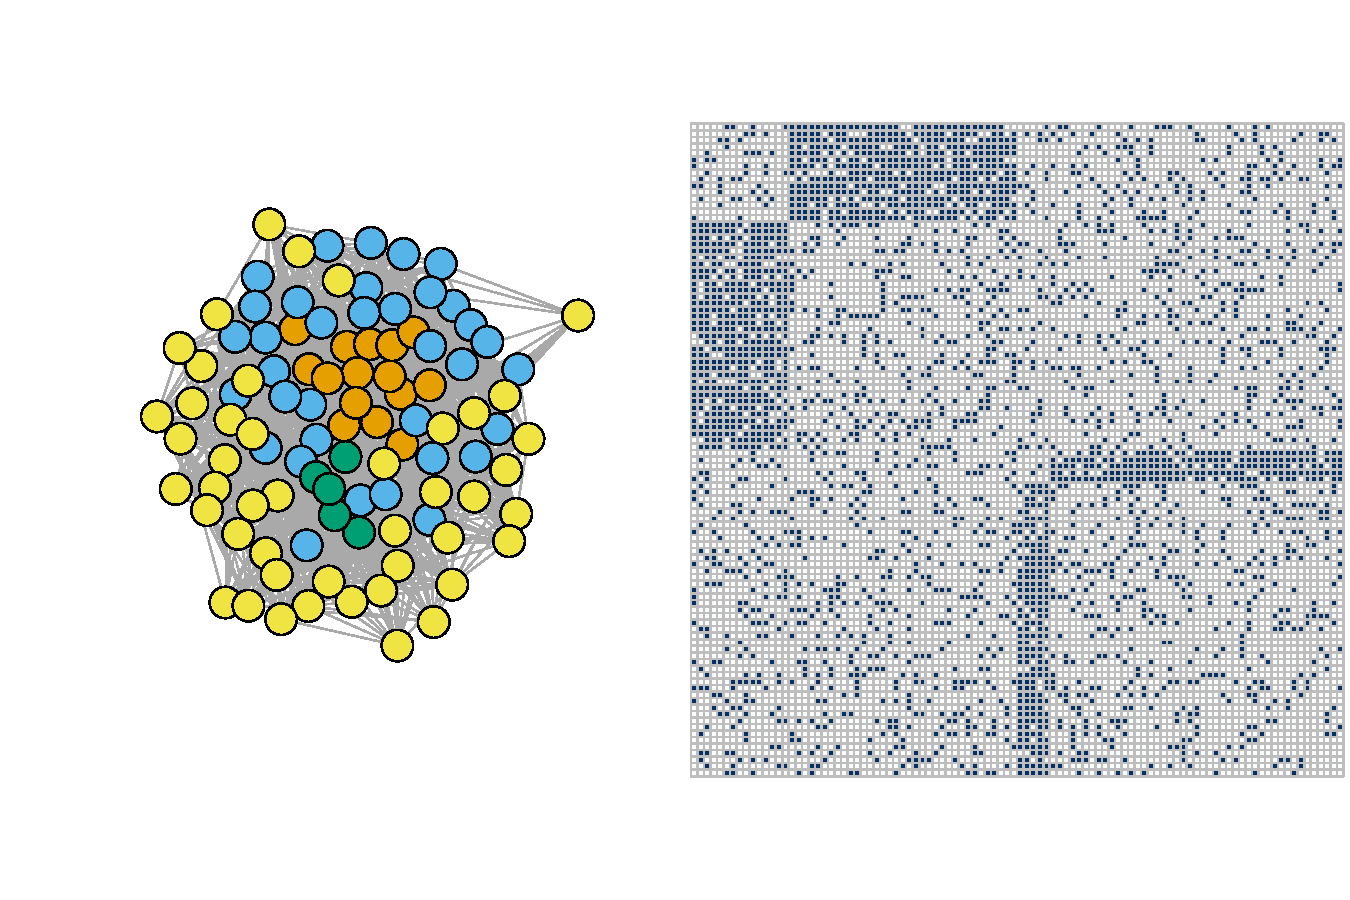
\includegraphics[width=.8\textwidth]{figures/unnamed-chunk-10-1} 
\end{knitrout}

\end{frame}



\begin{frame}
  \frametitle{Degree distributions}

  \begin{block}{Conditional degree distribution}
    The conditional degree distribution of a node $i\in q$ is
    \begin{equation*}
      D_i | i \in q \sim \mathrm{b}(n-1,\bar\pi) \approx \mathcal{P}(\lambda_q), \qquad \bar\pi_q = \sum_{\ell=1}^Q \alpha_\ell \pi_{q\ell}, \quad \lambda_q = (n-1)\bar\pi_q
    \end{equation*}
  \end{block}

  \vfill

  \begin{block}{Conditional degree distribution}
    The degree distribution of a node $i$ can be approximated by a mixture of Poisson distributions:
    \begin{equation*}
      \prob(D_i = k) = \sum_{q=1}^Q\alpha_q \exp{\set{-\lambda_q}} \ \frac{\lambda_q^k}{k !}
    \end{equation*}
  \end{block}

\end{frame}

%% ==========================================================================
\subsection{Statistical Inference in the SBM}
%% ==========================================================================

\begin{frame}
  \frametitle{Likelihoods}

\begin{block}{Complete data likelihood}
\vspace{-.5cm}
 \begin{align*}
\ell_c(\bY,\bZ; \theta)  & =  p(\bY | \bZ; \balpha) p(\bZ ; \boldsymbol\pi)\nonumber = \prod_{i,j} f_{\alpha_{Z_i,Z_j}}(Y_{ij}) \times   \prod_{i} \pi_{Z_i} \nonumber  \\
&=  \prod_{i,j} \alpha_{Z_i,Z_j}^{Y_{ij}} (1-  \alpha_{Z_i,Z_j})^{1- Y_{ij}}    \prod_{i} \pi_{Z_i} \nonumber
\end{align*}
 \end{block}
 
\begin{block}{Marginal likelihood $(\bY)$}
\vspace{-.5cm}
\begin{equation*}
\log \ell(\bY; \theta) =\log \sum_{\bZ \in \boldsymbol{\mathcal{Z}}} \ell_c(\bY,\bZ; \theta) \,.
\end{equation*}
$\boldsymbol{\mathcal{Z}} =   \{1,\dots, K\}^{n}$: impossible to compute  when  $K$ and $n$ increase. 
\end{block}

\vfill

\alert{Standard tool to maximize the likelihood when latent variables involved} : EM  algorithm.  
 
 \end{frame}


\begin{frame}{From EM to variational EM}

\begin{block}{Standard EM}
At iteration $(t)$ : 
\begin{itemize}
 \item[$\bullet$]\textbf{Step E}: compute 
 $$ Q(\theta | \theta^{(t-1)}) =   \mathbb E_{\bZ | \bY, \theta^{(t-1)} } \left[\log \ell_c(\bY,\bZ; \theta)  \right] $$
 \item[$\bullet$]\textbf{Step M}: 
 $$ \theta^{(t)} = \arg \max_{\theta} Q(\theta | \theta^{(t-1)})$$
 \end{itemize}
\end{block}

  With SBM,
    \begin{equation*}
      \E_{\bZ|\bY} \big[\log L(\btheta;\bX,\bZ) \big] = \sum_{i,q} \tau_{iq} \log \alpha_q + \sum_{i<j,q,\ell} \eta_{ijq\ell} \log \pi_{q\ell}^{X_{ij}} (1-\pi_{q\ell})^{1-X_{ij}}
    \end{equation*}
      where $\tau_ {iq}, \eta_{ijq\ell}$ are the posterior probabilities:
      \begin{itemize}
        \item $\tau_{iq} = \prob(Z_{iq} = 1 | \bX) = \E \left[Z_{iq} | \bX\right].$
        \item $\eta_{ijq\ell} = \prob(Z_{iq}Z_{j\ell} = 1 | \bX) = \E \left[Z_{iq}Z_{j\ell} | \bX\right].$
      \end{itemize}

\end{frame}

\begin{frame}
  \frametitle{The EM strategy does not apply directly for SBM}

  \begin{block}{Ouch: another intractability problem}
    \begin{itemize}
      \item the $Z_{iq}$ are \alert{not independent conditional on $(X_{ij}, i<j)$} \dots
      \item we cannot compute $\eta_{ijq\ell} = \prob(Z_{iq}Z_{j\ell} = 1 | \bX) = \E \left[Z_{iq}Z_{j\ell} | \bX\right]$,
      \item the conditional expectation $Q(\btheta)$, i.e. the main EM ingredient, is \alert{intractable}.
    \end{itemize}
  \end{block}

  \vfill

  \begin{block}{Solution: mean field approximation}
    Approximate $\eta_{ijq\ell}$ by $\tau_{iq}\tau_{j\ell}$, i.e., \alert{assume conditional independence between $Z_{iq}$}\\

    $\rightsquigarrow$ This can be formalized in the variational framework
  \end{block}


\end{frame}

\begin{frame}
  \frametitle{Revisting the EM algorithm I}

  \begin{proposition}
    Consider a distribution $\mathbb{Q}$ for the $\set{Z_{iq}}$. We have
    \begin{equation*}
      \log L(\btheta; \bX) = \E_{\mathbb{Q}} [\log L(\btheta, \bX,\bZ)] + \mathcal{H}(\mathbb{Q}) + \mathrm{KL}(\mathbb{Q} \ | \ \prob(\bZ|\bX;\btheta)),
    \end{equation*}
    where $\mathcal{H}$ is the entropy and $\mathrm{KL}( \cdot| \cdot)$ is the Kullback-Leibler divergence:
    \begin{gather*}
      \mathcal{H}(\mathbb{Q}) = - \sum_z \mathbb{Q}(z) \log \mathbb{Q}(z) = - \E_\mathbb{Q} [\log \mathbb{Q} (Z)]\\
      \mathrm{KL}(\mathbb{Q} \ | \ \prob(\bZ|\bX;\btheta)) = \sum_z \mathbb{Q}(z) \log \frac{\mathbb{Q}(z)}{\prob(\bZ|\bX;\btheta)} = \E_\mathbb{Q} \left[\log \frac{\mathbb{Q}(z)}{\prob(\bZ|\bX;\btheta)}\right]\\
    \end{gather*}
  \end{proposition}
\end{frame}

\begin{frame}
  \frametitle{Revisting the EM algorithm II}
  Let
   \begin{equation*}
    J(\mathbb{Q},\btheta) \triangleq \E_{\mathbb{Q}}\left(\log L(\btheta ;\bX,\bZ)\right) + \mathcal{H}(\mathbb{Q})
\end{equation*}

  \vfill

  The steps in the EM algorithm may be viewed as:
  \begin{description}
    \item[Expectation step]: choose $\mathbb{Q}$ to maximize $J(\mathbb{Q};\btheta^{(t)})$\\[2ex]
      \alert{The solution is $\prob(\bZ|\bX;\btheta^{(t)})$}\\
    \item[Maximization step]: choose $\btheta$ to maximize $J(\mathbb{Q}^{(t)};\btheta$)\\[2ex]
      \alert{The solution maximizes $\E_{\bZ|\bX;\btheta^{(t)}}\left(\log L(\btheta ;\bX,\bZ)\right)$}
  \end{description}

\end{frame}

\begin{frame}
  \frametitle{Variational approximation for SBM}

    \begin{block}{Problem for SBM}
      $\prob(\bZ|\bX;\btheta^{(t)})$ cannot be computed thus the E-step cannot be solved.
  \end{block}

  \begin{block}{Idea}
      Choose $\mathbb{Q}$ in a class of function so that the E-step can be solved.
  \end{block}

  \begin{block}{Family of distribution that factorizes}
      We chose $\mathbb{Q}$ the multinomial distribution so that
      \begin{equation*}
        \mathbb{Q}(\bZ) = \prod_{i=1}^n \mathbb{Q}_i(Z_i) = \prod_{i=1}^n\prod_{q=1}^Q \tau_{iq}^{Z_{iq}},
      \end{equation*}
      where $\tau_{iq} =\mathbb{Q}_i(Z_{i} = q) = \E_{\mathbb{Q}}(Z_{iq})$, with $\sum_{q} \tau_{iq} = 1$ for all $i=1,\dots,n$.
  \end{block}

\end{frame}

\begin{frame}
  \frametitle{Variational EM for SBM: the criterion}

  \begin{block}{Lower bound of the loglikehood}
  Since $\mathbb{Q}$ is an approximation of $\prob(\bZ|\bX)$, the Kullback-Leibler divergence is non-negative and
    \begin{equation*}
      \log L(\btheta; \bX) \geq \E_{\mathbb{Q}} [\log L(\btheta, \bX,\bZ)] + \mathcal{H}(\mathbb{Q}) = J(\mathbb{Q},\btheta).
    \end{equation*}
  \end{block}

  For the SBM,
  \begin{equation*}
  J(\mathbb{Q},\btheta) = \sum_{i,q} \tau_{iq} \log \alpha_q + \sum_{i<j,q,\ell}  \tau_{iq}  \tau_{j\ell} \log b(X_{ij} ; \pi_{q\ell}) - \sum_{i,q} \tau_{iq} \log(\tau_{iq}),
  \end{equation*}

  $\rightsquigarrow$ we optimize the loglikelihood lower bound $J(\mathbb{Q},\btheta) = J(\boldsymbol\tau,\btheta)$ in $(\boldsymbol\tau, \btheta)$.

\end{frame}

\begin{frame}
  \frametitle{E and M steps for SBM}

  \begin{block}{Variational E-step}
    Maximizing $J(\boldsymbol\tau)$ for fixed $\btheta$, we find a fixed-point relationship:
    \begin{equation*}
      \hat{\tau}_{iq} \varpropto \alpha_q \prod_{j} \prod_{\ell} b(X_{ij}, \pi_{q\ell})^{\hat{\tau}_{j\ell}}
    \end{equation*}
  \end{block}

  \vfill

  \begin{block}{M-step}
    Maximizing $J(\btheta)$ for fixed $\boldsymbol\tau$, we find,
    \begin{equation*}
\hat{\alpha}_q = \frac{1}{n}\sum_i \hat{\tau}_{iq} , \quad \hat\pi_{q\ell} = \frac{\sum_{i\neq j} \hat{\tau}_{iq}\hat{\tau}_{j\ell} X_{ij}}{\sum_{i\neq j} \hat{\tau}_{iq}\hat{\tau}_{j\ell}}.
\end{equation*}
  \end{block}

\end{frame}

\begin{frame}
  \frametitle{Model selection}

  We use our lower bound of the  loglikelihood to compute an approximation of the ICL
  \begin{multline*}
  \mathrm{vICL}(Q) = \E_{\hat{\mathbb{Q}}} [\log L(\hat{\btheta)};\bX,\bZ] \\ - \frac{1}{2} \left(\frac{Q(Q+1)}{2} \log \frac{n(n-1)}{2} + (Q-1) \log (n) \right),
\end{multline*}
where
    \begin{equation*}
      \E_{\hat{\mathbb{Q}}} [\log L(\hat\btheta; \bX,\bZ)] = J(\hat{\boldsymbol\tau},\hat\btheta) - \mathcal{H}(\hat{\mathbb{Q}}).
    \end{equation*}

    The variational BIC is just
    \begin{equation*}
  \mathrm{vBIC}(Q) = J(\hat{\boldsymbol\tau},\hat\btheta) - \frac{1}{2} \left(\frac{Q(Q+1)}{2} \log \frac{n(n-1)}{2} + (Q-1) \log (n) \right).
    \end{equation*}

\end{frame}


\begin{frame}[fragile]
    \frametitle{Example: French politcal blogosphere}
    


\begin{knitrout}\scriptsize
\definecolor{shadecolor}{rgb}{0.969, 0.969, 0.969}\color{fgcolor}\begin{kframe}
\begin{alltt}
\hlstd{my_sbm} \hlkwb{<-}
  \hlstd{blog} \hlopt \hlkwd{as_adj}\hlstd{(}\hlkwc{sparse} \hlstd{=} \hlnum{FALSE}\hlstd{)} \hlopt
   \hlstd{sbm}\hlopt{::}\hlkwd{estimateSimpleSBM}\hlstd{(}\hlkwc{estimOptions} \hlstd{=} \hlkwd{list}\hlstd{(}\hlkwc{plot} \hlstd{=} \hlnum{FALSE}\hlstd{))}
\end{alltt}
\end{kframe}
\end{knitrout}

\begin{knitrout}\scriptsize
\definecolor{shadecolor}{rgb}{0.969, 0.969, 0.969}\color{fgcolor}\begin{kframe}
\begin{alltt}
\hlstd{my_sbm}
\end{alltt}
\begin{verbatim}
## Fit of a Simple Stochastic Block Model -- bernoulli variant
## =====================================================================
## Dimension = ( 192 ) - ( 10 ) blocks and no covariate(s).
## =====================================================================
## * Useful fields 
##   $nbNodes, $modelName, $dimLabels, $nbBlocks, $nbCovariates, $nbDyads
##   $blockProp, $connectParam, $covarParam, $covarList, $covarEffect 
##   $expectation, $indMemberships, $memberships 
## * R6 and S3 methods 
##   $rNetwork, $rMemberships, $rEdges, plot, print, coef 
## * Additional fields
##   $probMemberships, $loglik, $ICL, $storedModels, 
## * Additional methods 
##   predict, fitted, $setModel, $reorder
\end{verbatim}
\end{kframe}
\end{knitrout}


    
\end{frame}

\begin{frame}[fragile]
    \frametitle{Example: model exploration (vICL)}

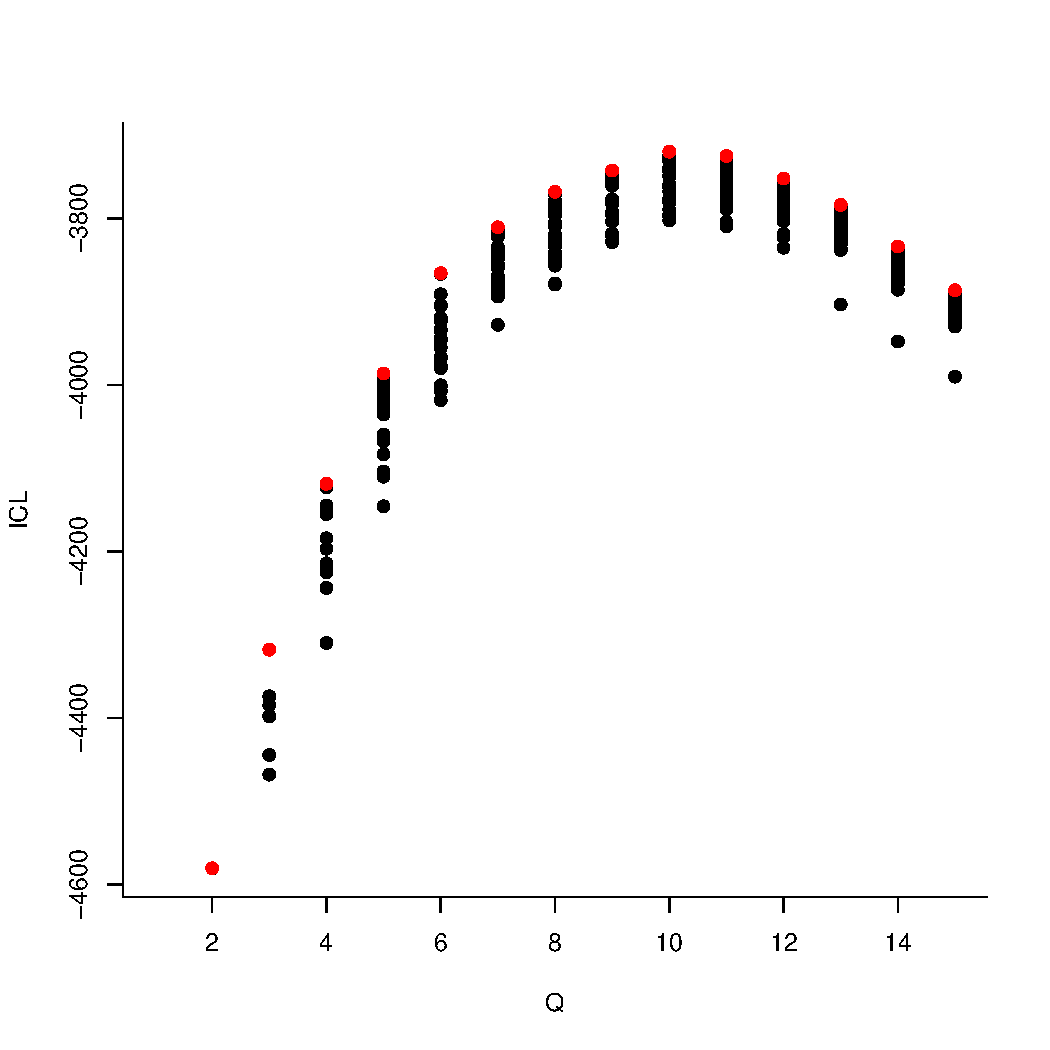
\includegraphics[width=.7\textwidth]{figures/ICL_fblog}

\end{frame}

\begin{frame}[fragile]
    \frametitle{Example: monitoring convergence (ELBO)}



\begin{knitrout}\scriptsize
\definecolor{shadecolor}{rgb}{0.969, 0.969, 0.969}\color{fgcolor}
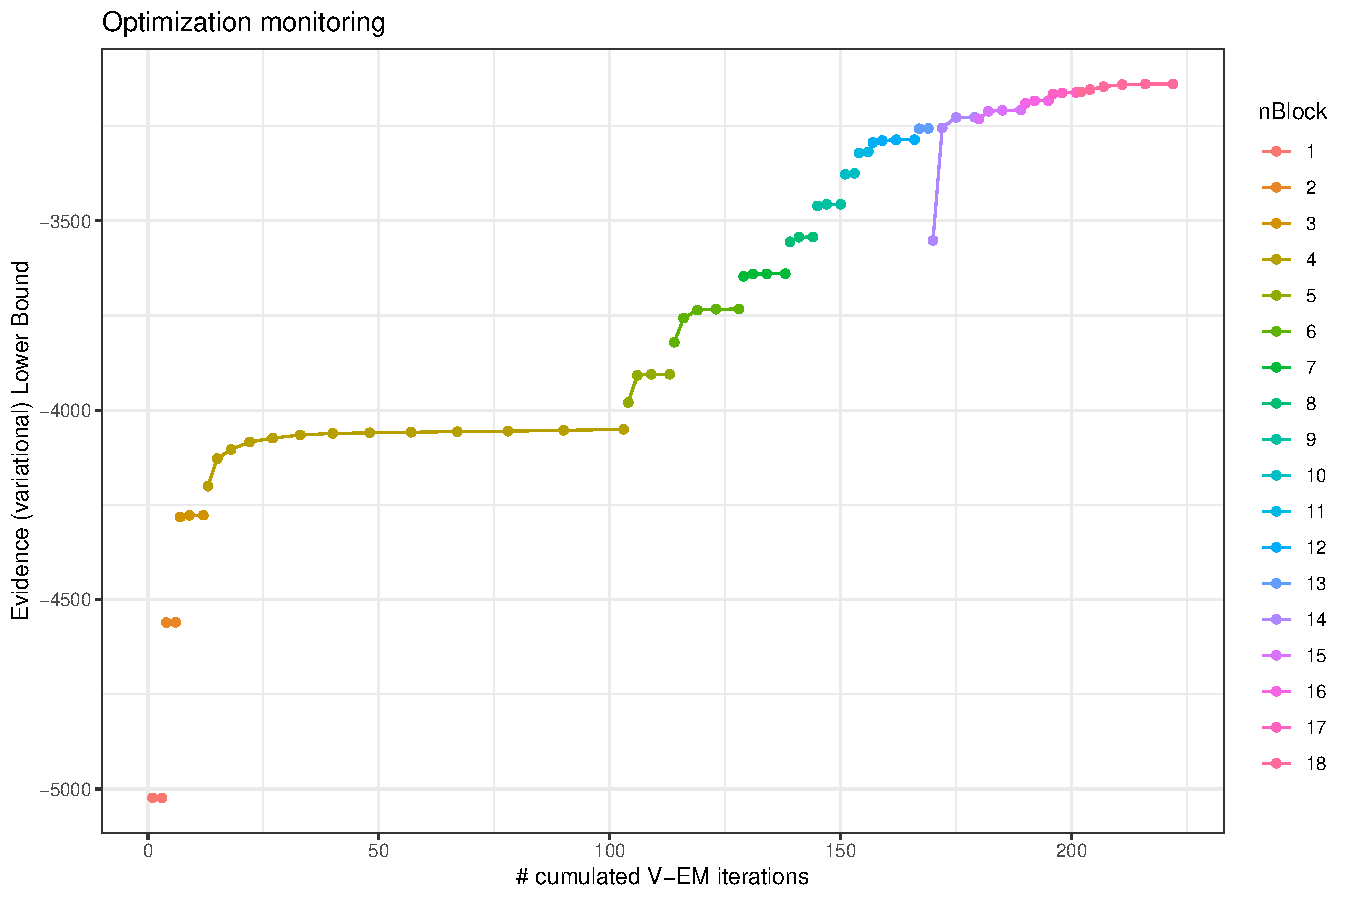
\includegraphics[width=.8\textwidth]{figures/unnamed-chunk-14-1} 
\end{knitrout}

\end{frame}

\begin{frame}[fragile]
  \frametitle{Vizualisation: matrix view}

\begin{knitrout}\scriptsize
\definecolor{shadecolor}{rgb}{0.969, 0.969, 0.969}\color{fgcolor}\begin{kframe}
\begin{alltt}
\hlkwd{plot}\hlstd{(my_sbm,} \hlkwc{dimLabels} \hlstd{=} \hlkwd{list}\hlstd{(}\hlkwc{row} \hlstd{=} \hlstr{"blogs"}\hlstd{,} \hlkwc{col} \hlstd{=} \hlstr{"blogs"}\hlstd{))}
\end{alltt}
\end{kframe}
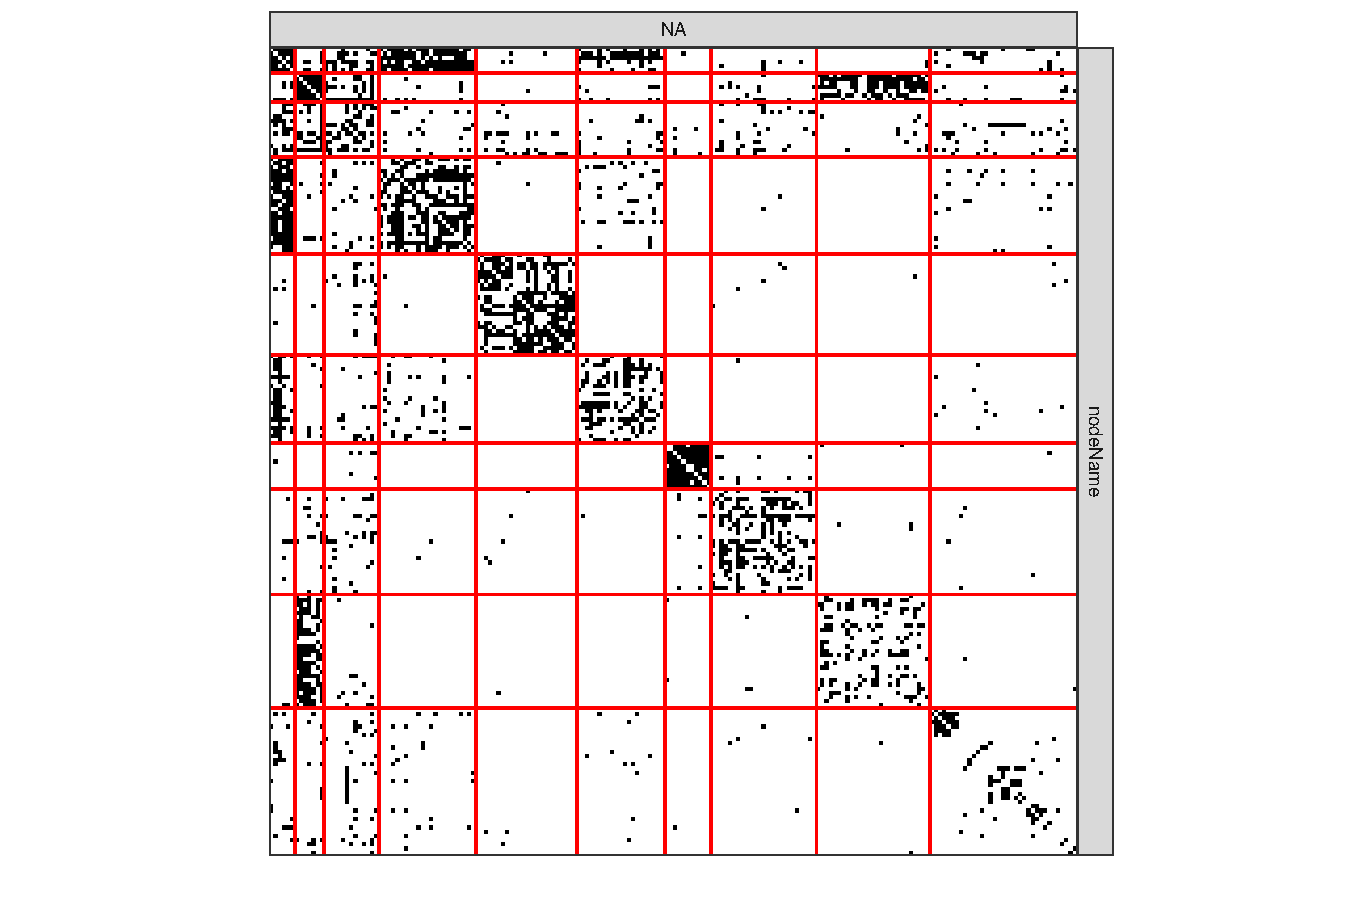
\includegraphics[width=.8\textwidth]{figures/unnamed-chunk-15-1} 
\end{knitrout}

\end{frame}

\begin{frame}[fragile]
  \frametitle{Vizualisation: expected value}

\begin{knitrout}\scriptsize
\definecolor{shadecolor}{rgb}{0.969, 0.969, 0.969}\color{fgcolor}\begin{kframe}
\begin{alltt}
\hlkwd{plot}\hlstd{(my_sbm,} \hlstr{"expected"}\hlstd{,} \hlkwc{dimLabels} \hlstd{=} \hlkwd{list}\hlstd{(}\hlkwc{row} \hlstd{=} \hlstr{"blogs"}\hlstd{,} \hlkwc{col} \hlstd{=} \hlstr{"blogs"}\hlstd{))}
\end{alltt}
\end{kframe}
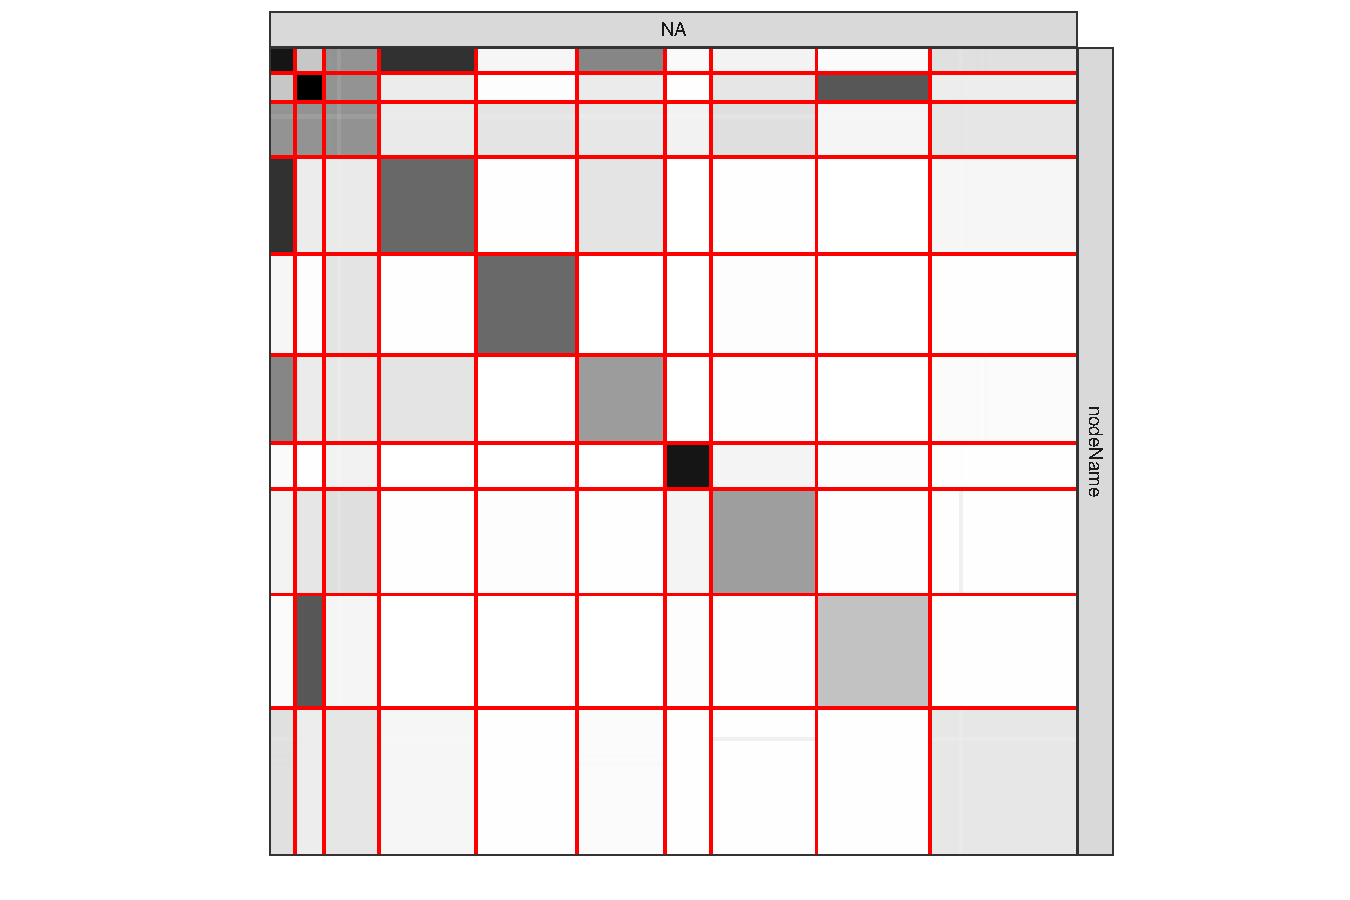
\includegraphics[width=.8\textwidth]{figures/unnamed-chunk-16-1} 
\end{knitrout}

\end{frame}

\begin{frame}[fragile]
  \frametitle{Vizualisation: mesoscopic view}

\begin{knitrout}\scriptsize
\definecolor{shadecolor}{rgb}{0.969, 0.969, 0.969}\color{fgcolor}\begin{kframe}
\begin{alltt}
\hlkwd{plot}\hlstd{(my_sbm,} \hlstr{"meso"}\hlstd{)}
\end{alltt}
\end{kframe}
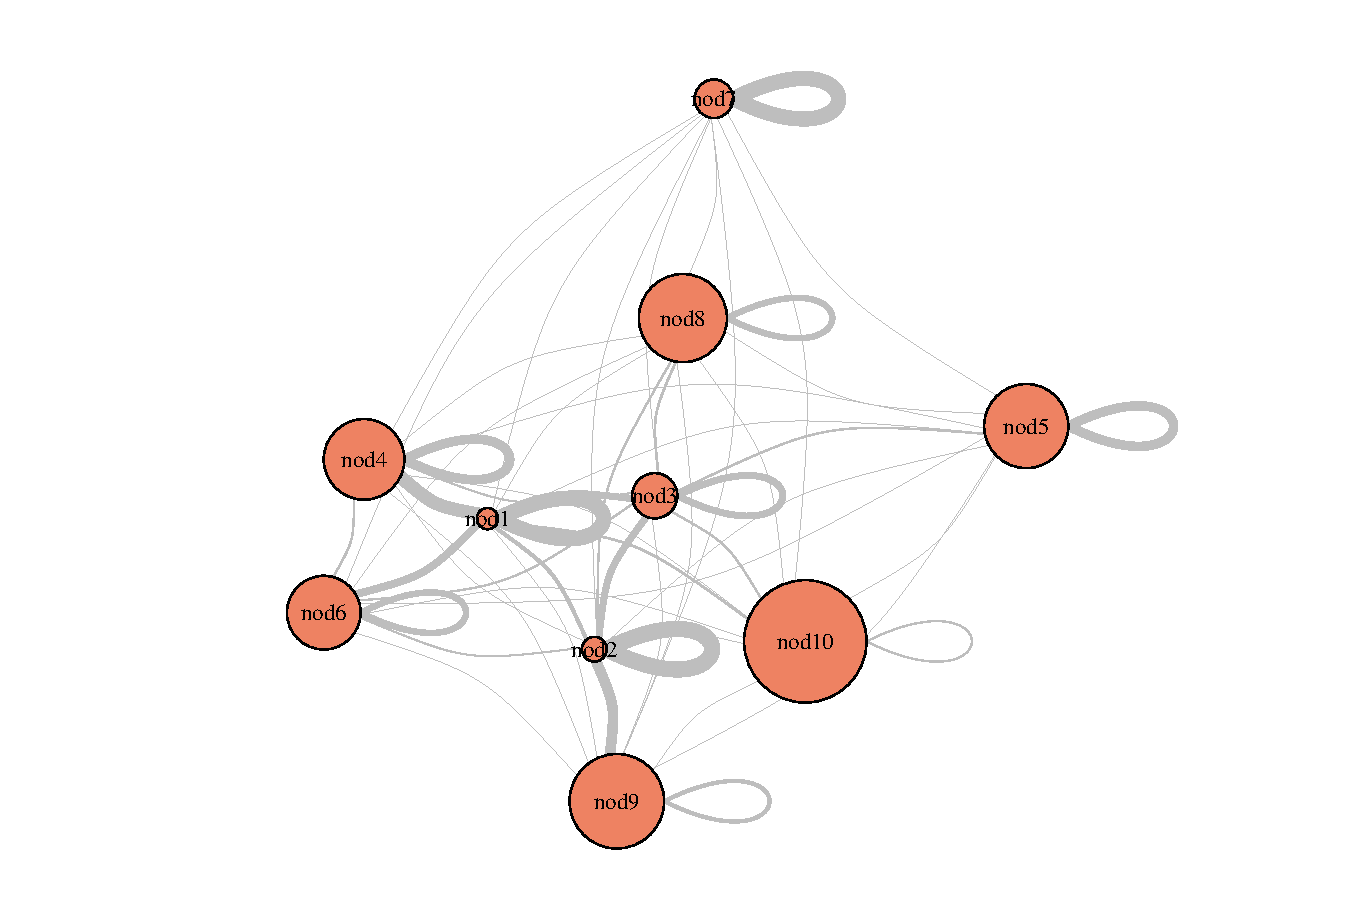
\includegraphics[width=.8\textwidth]{figures/unnamed-chunk-17-1} 
\end{knitrout}


\end{frame}

\begin{frame}[fragile,allowframebreaks]
  \frametitle{Accessing field}

\begin{knitrout}\scriptsize
\definecolor{shadecolor}{rgb}{0.969, 0.969, 0.969}\color{fgcolor}\begin{kframe}
\begin{alltt}
\hlstd{aricode}\hlopt{::}\hlkwd{ARI}\hlstd{(my_sbm}\hlopt{$}\hlstd{memberships, party)}
\end{alltt}
\begin{verbatim}
## [1] 0.4650112
\end{verbatim}
\end{kframe}
\end{knitrout}

\begin{knitrout}\scriptsize
\definecolor{shadecolor}{rgb}{0.969, 0.969, 0.969}\color{fgcolor}\begin{kframe}
\begin{alltt}
\hlkwd{barplot}\hlstd{(my_sbm}\hlopt{$}\hlstd{blockProp)}
\end{alltt}
\end{kframe}
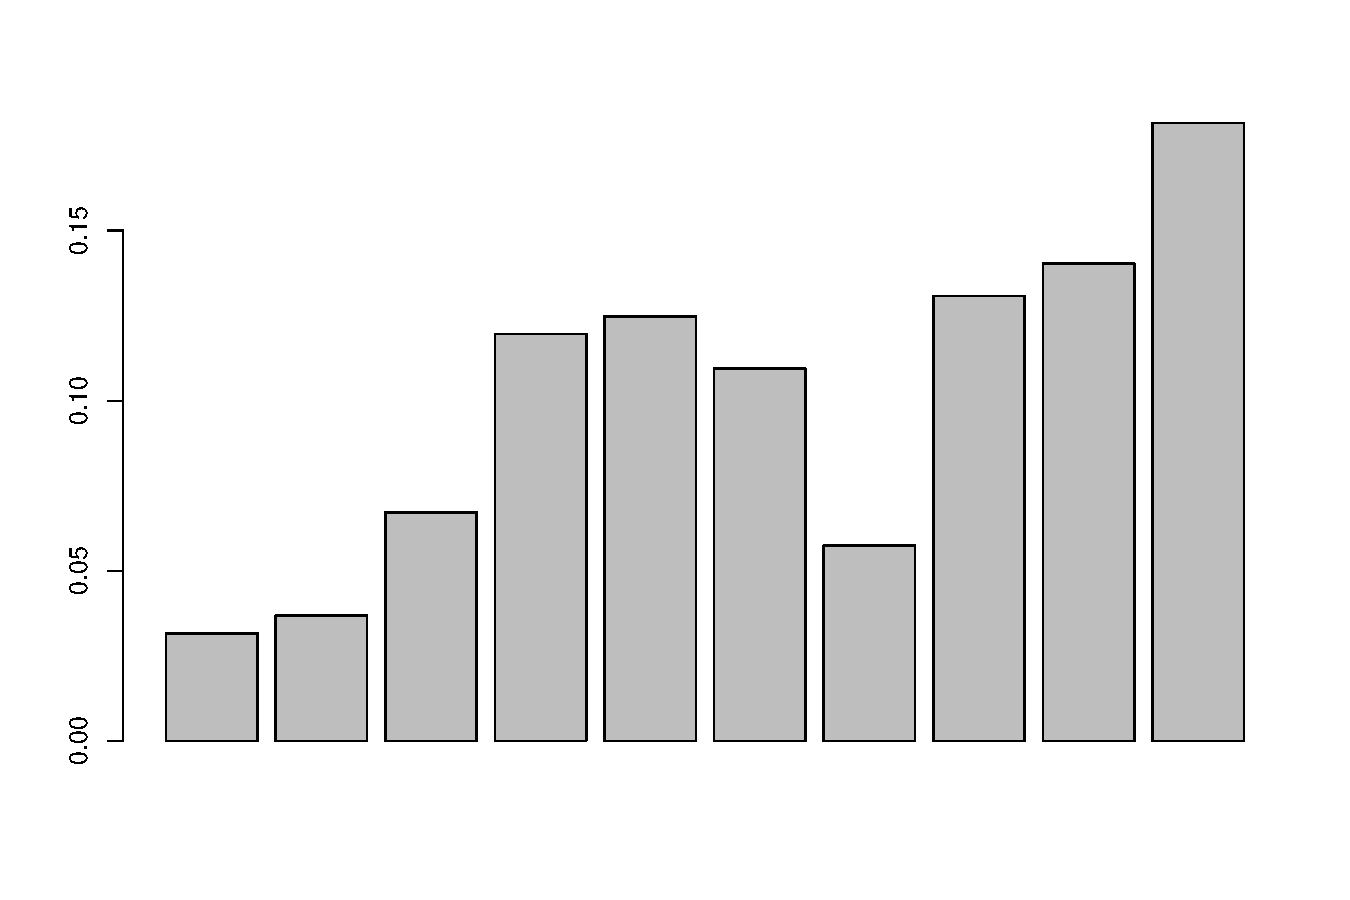
\includegraphics[width=.8\textwidth]{figures/unnamed-chunk-19-1} 
\end{knitrout}

\begin{knitrout}\scriptsize
\definecolor{shadecolor}{rgb}{0.969, 0.969, 0.969}\color{fgcolor}\begin{kframe}
\begin{alltt}
\hlkwd{corrplot}\hlstd{(my_sbm}\hlopt{$}\hlstd{connectParam}\hlopt{$}\hlstd{mean)}
\end{alltt}
\end{kframe}
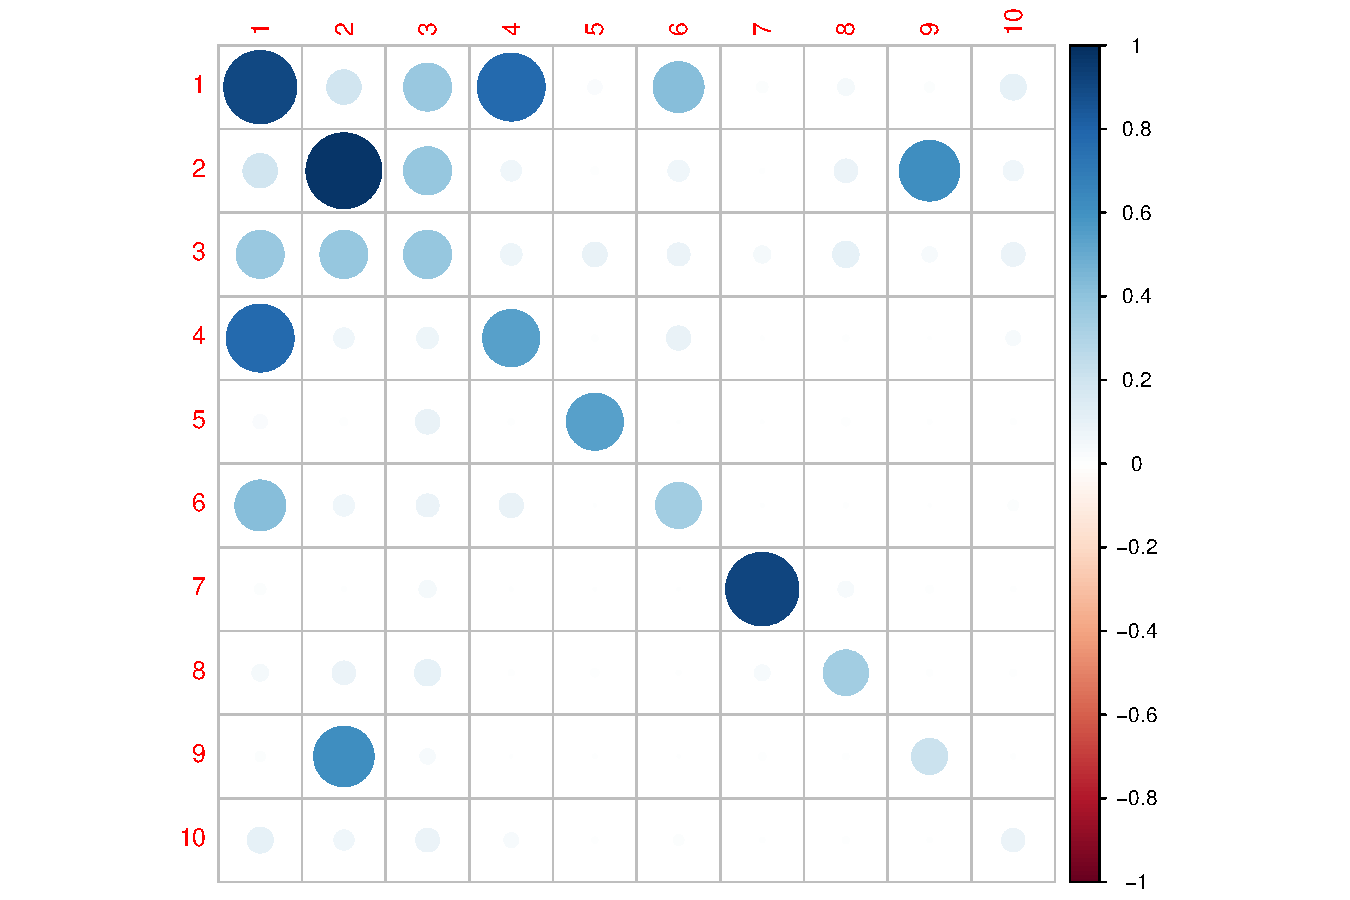
\includegraphics[width=.8\textwidth]{figures/unnamed-chunk-20-1} 
\end{knitrout}

etc... see documentation and website

\end{frame}

\subsection{SBM: some extensions}

\begin{frame}
 \frametitle{SBM with covariates}

\begin{itemize}
\item As before :  ($Y_{ij}$) be an adjacency matrix 
\item  Let   $x^{ij} \in \mathbb{R}^p$  denote covariates describing the pair $(i,j)$
\end{itemize}

\begin{block}{Latent variables : as before }
\begin{itemize}
\item The nodes $i= 1,\dots,n$ are partitioned into $K$ clusters
\item $Z_i$ independent variables $ \mathbb{P}(Z_i = k) = \pi_k$
\end{itemize}
\end{block}
 
\begin{block}{Conditionally to $(Z_i)_{i=1,\dots,n}$... }

$(Y_{ij})$ independent and 
\begin{eqnarray*}
 Y_{ij}  | Z_i, Z_j&\sim&   \mathcal{B}ern(\mbox{logit}(\alpha_{Z_i,Z_j} + \theta \cdot x_{ij}) ) \quad \mbox {if binary data} \\
 Y_{ij}  | Z_i, Z_j  &\sim&  \mathcal{P}(\exp(\alpha_{Z_i,Z_j} + \theta  \cdot x_{ij}) ) \quad \mbox {if counting data} 
\end{eqnarray*}
\end{block}


If $K = 1$ : all the connection heterogeneity is explained by the covariates. 
 \end{frame}

\begin{frame}
 \frametitle{Valued-edge networks}
 

\begin{block}{Values-edges networks}
 Information on edges can be something different from presence/absence.
 It can be:
 \begin{enumerate}
  \item a count of the number of observed interactions,
  \item a quantity interpreted as the interaction strength,
  \end{enumerate}

 \end{block}

 \bigskip
 
 


\begin{block}{ Natural extensions of SBM and LBM}
 \begin{enumerate}
  \item Poisson distribution: $Y_{ij} \ | \ \{i\in\textcolor{yellow!40!orange}{\bullet},j\in\textcolor{blue!80!black}{\bullet}\}
\sim^{\text{ind}} \mathcal{P}(\lambda_{\textcolor{yellow!40!orange}{\bullet}\textcolor{blue!80!black}{\bullet}})$,
 \item Gaussian distribution: $Y_{ij} \ | \ \{i\in\textcolor{yellow!40!orange}{\bullet},j\in\textcolor{blue!80!black}{\bullet}\}
\sim^{\text{ind}} \mathcal{N}(\mu_{\textcolor{yellow!40!orange}{\bullet}\textcolor{blue!80!black}{\bullet}},\sigma^2)$,
\textcolor{mygreen}{\cite{mariadassou2010uncovering}}
\item More generally, 
  $$Y_{ij} \ | \ \{i\in\textcolor{yellow!40!orange}{\bullet},j\in\textcolor{blue!80!black}{\bullet}\}
\sim^{\text{ind}} \mathcal{F}(\theta_{\textcolor{yellow!40!orange}{\bullet}\textcolor{blue!80!black}{\bullet}})$$
 \end{enumerate}
 \end{block}
 \bigskip

\end{frame}

\begin{frame}{Latent Block Models aka Bipartite SBM}

Let $Y_{ij}$ be a bi-partite network. Individuals in row and cols are not the same. 

\begin{block}{Latent variables : bi-clustering}
\begin{itemize}
\item Nodes $i= 1,\dots,n_1$   partitionned into $K_1$ clusters,  nodes $j= 1,\dots,n_2$  partitionned into $K_2$ clusters
\item $$\begin{array}{cl}
Z^1_i = k & \mbox{if node $i$ belongs to cluster (block) $k$}\\
Z^2_j = \ell & \mbox{if node $j$ belongs to cluster (block) $\ell$}
\end{array}$$
\item $Z^1_i, Z^2_j$ independent variables
$$ \mathbb{P}(Z^1_i = k) = \pi^1_k,\quad  \mathbb{P}(Z^2_j = \ell) = \pi^2_\ell$$
\end{itemize}
\end{block}

\end{frame}

\begin{frame}
\frametitle{Latent Block Model : illustration}

 \begin{center}
    \begin{overlayarea}{\textwidth}{.5\textheight}
      \begin{columns}
        \begin{column}{.45\paperwidth}
        \centering
        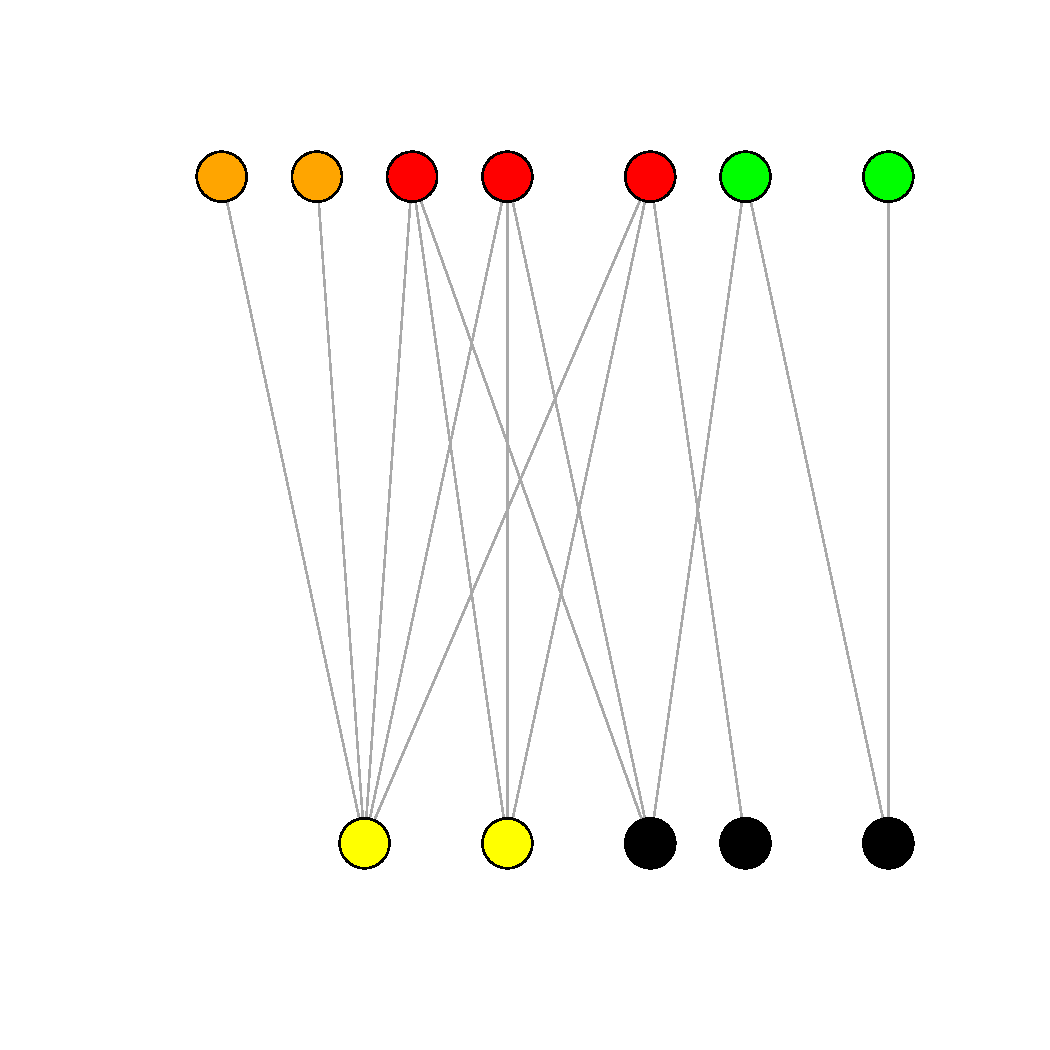
\includegraphics[scale=.3]{figures/LBM_example.pdf}
        \end{column}
        \begin{column}{.5\paperwidth}
          \begin{small}
            \begin{block}{Latent Block Model}
              \begin{itemize}
              \item
                $n_1$ row nodes $\mathcal{K}_1=\{\textcolor{red}{\bullet},\textcolor{orange}{\bullet},\textcolor{green}{\bullet}\}$
                classes
              \item  $\pi^1_\bullet  =  \mathbb{P}(i  \in  \bullet)$,
                $\bullet\in\mathcal{K}_1,i=1,\dots,n$
              \item $n_2$ column nodes $\mathcal{K}_2=\{\textcolor{yellow}{\bullet},\textcolor{black}{\bullet}\}$
                classes
               \item  $\pi^2_\bullet  =  \mathbb{P}(j  \in  \bullet)$,
                $\bullet\in\mathcal{K}_2,j=1,\dots,m$
              \item      $\alpha_{\textcolor{red}{\bullet}\textcolor{yellow}{\bullet}}     =      \mathbb{P}(i
                \leftrightarrow j | i\in\textcolor{red}{\bullet},j\in\textcolor{yellow}{\bullet})$
              \end{itemize}
            \end{block}
          \end{small}
        \end{column}
      \end{columns}
    \end{overlayarea}
  \end{center}


\begin{align*}
Z^1_i = \mathbf{1}_{\{i \in \bullet\}}  \ & \sim^{\text{iid}} \mathcal{M}(1,\boldsymbol\pi^1), \quad \forall\bullet \in \mathcal{Q}_1, \\ 
Z^2_j=\mathbf{1}_{\{j \in \bullet\}}  \ & \sim^{\text{iid}} \mathcal{M}(1,\boldsymbol\pi^2), \quad \forall\bullet \in \mathcal{Q}_2, \\
Y_{ij} \ | \ \{i\in\textcolor{red}{\bullet},j\in\textcolor{yellow}{\bullet}\}
& \sim^{\text{ind}} \mathcal{B}ern(\alpha_{\textcolor{red}{\bullet}\textcolor{yellow}{\bullet}})\\
\end{align*}

\end{frame}

\begin{frame}
  \frametitle{To go further...}
  
  \begin{itemize}
    \item Group Gro{\ss}BM : \url{https://github.com/GrossSBM/}  \texttt{sbm}; 
    \item Documentation of package \texttt{sbm}: \url{https://grosssbm.github.io/sbm/}
    \item \texttt{missSBM} SBM with missing data \url{https://github.com/GrossSBM/misssbm} \\
    
      Slides : \url{https://grosssbm.github.io/slideshow-missSBM/slides.html}

  \end{itemize}
    
\end{frame}

\end{document}
